%%% Dateikodierung: UTF-8
%%% äöüÄÖÜß  <-- keine deutschen Umlaute hier? UTF-faehigen Editor verwenden!

%%% Magic Comments zum Setzen der korrekten Parameter in kompatiblen IDEs
% !TeX encoding = utf8
% !TeX program = pdflatex 
% !TeX spellcheck = de_DE
% !BIB program = biber

\RequirePackage[utf8]{inputenc} % bei Verw. von lualatex oder xelatex entfernen!
\RequirePackage{hgbpdfa}        % Erzeugt ein PDF/A-2b-konformes Dokument

\documentclass[bachelor,german,smartquotes,alphabetic]{hgbthesis}
% Zulässige Optionen in [..]: 
%    Typ der Arbeit: 'diploma', 'master' (default), 'bachelor', 'internship'
%		 Zusätzlich für ein Thesis-Exposé: 'proposal' (für 'bachelor' und 'master')
%    Hauptsprache: 'german' (default), 'english'
%    Option zur Umwandlung in typografische Anführungszeichen: 'smartquotes'
%    APA Zitierstil: 'apa'
%%%-----------------------------------------------------------------------------

\usepackage{listings}
\usepackage{xcolor}

\graphicspath{{images/}}  % Verzeichnis mit Bildern und Grafiken
\logofile{logo}           % Logo-Datei: images/logo.pdf (kein Logo: \logofile{})
\bibliography{references} % Biblatex-Literaturdatei (references.bib)
\usepackage{hyperref}
\usepackage[acronym]{glossaries}

\makeglossaries

\newacronym{jvm}{JVM}{Java Virtual Machine}
\newacronym{vt}{VT}{Virtual Thread}
\newacronym{pt}{PT}{Plattform Thread}
\newacronym{ot}{OT}{Betriebssystem Thread}
\newacronym{sts}{STS}{StructuredTaskScope}                          % makeglossaries main in der cmd ausführen

%%%-----------------------------------------------------------------------------
\begin{document}
%%%-----------------------------------------------------------------------------


\includepdf[pages=-]{Titelblatt.pdf}

%%%-----------------------------------------------------------------------------
% Angaben für die Titelei (Titelseite, Erklärung etc.)
%%%-----------------------------------------------------------------------------

\title{Virtuelle Threads und strukturierte Nebenläufigkeitssteuerung in Java}
\author{Gernot Hofbauer}
\programname{Software Engineering}

%\programtype{Fachhochschul-Bachelorstudiengang} % auswählen/editieren
\programtype{Fachhochschul-Bachelorstudiengang}

\placeofstudy{Hagenberg}
\dateofsubmission{2024}{06}{25} % {YYYY}{MM}{DD}

% \advisor{Dr. Alois B.~Treuer} % optional %
% \advisor{FH-Prof. DI Johann Heinzelreiter}


%\strictlicense % restriktive Lizenz anstatt Creative Commons (nicht empfohlen!)

%%%-----------------------------------------------------------------------------
\frontmatter                                       % Titelei (röm. Seitenzahlen)
%%%-----------------------------------------------------------------------------

% \maketitle

% \chapter{Vorwort}

 % Ein Vorwort ist optional
\chapter{Kurzfassung}

    Diese Bachelorarbeit befasst sich mit einigen Neuerungen von \emph{Project Loom} für Java. Es wird detailliert auf \emph{virtuelle Threads}, \emph{StructuredTaskScopes},
    die auch auf virtuellen Threads basieren
    und \emph{ScopedValues} eingegangen.
    Zu jeder dieser Technologien wird zunächst eine technische Übersicht geboten, bei der darauf eingegangen wird, inwiefern sie sich von den bereits bekannten Technologien unterscheiden.
    Darauf folgt eine eine Erklärung, wie sie in Java verwendet werden können, wobei einige Beispiele gezeigt werden. 
    Bei \texttt{StructuredTaskScopes} beinhaltet dies auch das Einbinden eigener Logik und Fehlerbehandlung durch Ableitung von der Basisklasse. Bei \texttt{ScopedValues} wird auch auf die Unterschiede zu \texttt{ThreadLocal} eingegangen. 
    Um eine besseren Vergleich zwischen den bekannten Technologien und den Neuerungen von Projekt Loom ziehen zu können, wird das Laufzeitverhalten eingehend analysiert. Dazu wurden sechs einfache Benchmarks,
    welche das Laufzeitverhalten untersuchen, erstellt und durchgeführt. Aufgrund von Schwierigkeiten
    beim Messen des Speicherverbrauchs wurde zu diesem Aspekt nur ein Test durchgeführt. Die Messergebnisse wurden ausführlich analysiert und interpretiert.
    Dabei wurde festgestellt, dass virtuelle Threads in in den meisten Fällen Plattform-Threads überlegen sind. Lediglich bei wenigen, stark rechenintensiven Aufgaben, ganz ohne blockierende Aufrufe, 
    sollten Plattform-Threads bevorzugt werden. Eine der größten Stärken von virtuellen Threads ist die Möglichkeit, in sehr großen Mengen, ohne viel Overhead erstellt zu werden. 
    Dadurch skalieren sie besser und sind leichtgewichtiger als Plattform-Threads.
    ScopedValues sind bei der Vererbung von Werten über Threads hinweg schneller als ThreadLocal und benötigen bei großen Mengen an Threads wesentlich weniger Speicher. 
    Sie können daher in Kombination mit virtuellen Threads sehr empfohlen werden. Die Wertabfrage selbst ist aber ein wenig langsamer als bei ThreadLocal.
    Im Gegensatz zu ThreadLocal sind ScopedValues nicht veränderbar und können somit nicht immer als Ersatz verwendet werden.
		
\chapter{Abstract}

\begin{english}
Large Public Display Games place several specific design requirements. Such
games need to work equally well for just a few or several simultaneous users.
Also, entering, leaving, or joining a game in progress should be easily possible
without interrupting the game's flow. This bachelor (master) thesis focuses on
developing a game mechanics framework that supports the principle of smooth
transition gameplay. This framework will then be evaluated utilizing a prototype
implemented in a term project.
\end{english}
			
\printglossary[type=\acronymtype,title=Akronyme]
\tableofcontents

%%%-----------------------------------------------------------------------------
\mainmatter                             % Hauptteil (ab hier arab. Seitenzahlen)
%%%-----------------------------------------------------------------------------

\chapter{Einleitung}
\label{cha:Einleitung}

    Seit einigen Jahren Arbeitet Oracle an Möglichkeiten zur Verbesserung der Skalierbarkeit von Java-Anwendungen im Projekt "Loom".
    Der Hauptansatz dieses Vorhabens ist die Einführung von virtuellen Threads, die von der JVM verwaltet werden. 
    Diese Threads sind leichtgewichtiger als klassische Plattform Threads und können in größerer Anzahl erzeugt werden.
    So können bestimmte Anwendungen mit hoher Nebenläufigkeit zukünftig effizienter gestaltet werden. Diese Bachelorarbeit 
    beleuchtet diese Technologien und stellt die Neuerungen dem bereits Bekanntem gegenüber.

\section{Ziel der Arbeit}
\label{sec:Ziel}

    Das Ziel dieser Bachelorarbeit ist es, die grundlegenden Eigenschaften und Limitierungen des bestehenden Thread-Konzepts zu untersuchen und die Motivationen für die Neuerungen
    durch Projekt Loom zu verstehen. Ein Überblick über Projekt Loom und die damit verbundenen Technologien wird gegeben, wobei der Schwerpunkt auf Virtual Threads liegt. 
    Die Arbeit soll zeigen, wie und in welchen Fällen diese Neuerungen in der Praxis angewendet werden können und welche neuen Möglichkeiten sich dadurch ergeben. 
    Es wird auch verdeutlicht, welche bestehenden Probleme der parallelen Ausführung durch die neuen Technologien nicht gelöst werden können. 
    Durch Benchmarks sollen Laufzeit und Speicherverbrauch unter verschiedenen Umständen analysiert werden, um daraus Schlüsse zu ziehen, 
    in welchen Fällen die neuen Technologien verwendet werden sollten und in welchen nicht. Als konkretes Ergebnis wird eine Sammlung kleinerer Programme erstellt, 
    die die neuen Technologien in Projekt Loom demonstrieren und die Unterschiede zu den bisherigen Technologien aufzeigen.




\chapter{Das derzeitige Threadmodell}
\label{cha:DasDerzeitigeThreadmodell}                   % 5 Seiten
    Java und die \gls{jvm} stellen mit der Klasse \texttt{Thread} und dem Interface \texttt{Runnable} im Paket \texttt{java.lang} grundlegende Mechanismen zur Thread-Verarbei\-tung bereit.
    Mit dem Start der JVM werden automatisch der Haupt-Thread und administrative Threads wie der Garbage Collector gestartet. Jeder Thread kann seinerseits weitere Threads instanziieren \cite{GrundKursBS}.
  
\section{Funktionsweise}                                         
\label{sec:Funktionsweise}

    Bisher war jeder Thread in der \gls{jvm} eine Instanz von \texttt{java.lang.Thread}, auch \gls{pt} genannt. Diese Klasse stellt eine Wrapper-Klasse um \Glspl{ot} dar und Instanzen dieser Klasse
    binden den darunterliegenden \gls{ot}  während ihrer gesamten Lebenszeit an sich. Dadurch ist die Anzahl der gesamt verfügbaren \Glspl{pt} durch die Anzahl der \Glspl{ot} begrenzt und die Verwaltung
    der Ressourcen wie CPU-Rechenzeit unterliegt dem Betriebssystem \cite{JEP425}.
    \texttt{java.lang.Thread} implementiert die Schnittstelle \texttt{Runnable} und lässt Ableitungen zu.
    Außerdem können sogenannte \emph{Thread-Pools} genutzt werden. Dabei handelt es sich um einen Mechanismus, der mehrere \texttt{worker-threads} verwaltet. Diese existieren unabhängig von dem \texttt{Runnable},
    das sie ausführen. Die Verwendung von Thread-Pools verringert den Overhead, der sich durch die Erstellung von Threads ergibt \cite{ThreadPool}. Thread-Pools können über die Konstruktoren der Klasse 
    \texttt{ThreadPoolExecutor}
    erstellt werden, es ist jedoch üblich auf die Factory-Methoden der Klasse \texttt{Executors} zurückzugreifen. Die Methode \texttt{newFixedThreadPool(int nThreads)} ermöglicht es, 
    die Menge an Threads konstant zu halten. Wird ein Thread beendet, durch einen Fehler oder Abschluss der Arbeit, erstellt der Pool sofort einen neuen. Andere Implementierungen wie der 
    \texttt{newThread\-PerTaskExecutor} versuchen für jede Aufgabe einen eigenen Thread zu erstellen. Alle Aufgaben, die nicht direkt bearbeitet werden können, 
    speichert der Thread-Pool in einem Behälter zwischen. Thread-Pools müssen nach der Verwendung wieder geschlossen werden. Entweder mittels \texttt{shutdown()} oder der Verwendung eines
    try-with-resources-Blocks.
    Die \gls{jvm} kann bei Verwendung eines \texttt{CachedThreadPool}s Threads, die ihre Arbeit bereits 
    abgeschlossen haben, wiederverwenden, um eine neue Instanziierung zu vermeiden. Dabei werden Threads, die ihre Aufgabe bereits abgeschlossen haben, für weitere 60 Sekunden am Leben erhalten um 
    neue Aufgaben darauf ausführen zu können. Erst danach werden sie freigegeben. Natürlich können bei Bedarf neue Threads erstellt werden \cite{Executors}.

    
\section{Probleme}                                         
\label{sec:Probleme}

    \Glspl{ot} bringen viele Probleme mit sich. Eines der größten ist deren Ressourcenintensität.
    Sie müssen alle verschiedene Sprachen und Aufgaben unterstützen. Es ist wichtig, dass sie die Ausführung eines Prozesses unterbrechen und
    wiederaufnehmen können, 
    was das Speichern des Zustands (z.B. des Stack-Pointers und des Program-Counters) erfordert. Da das Betriebssystem keine Informationen darüber hat, wie
    eine Sprache ihren Stapel verwaltet, wird der Speicher großzügig zugeteilt und kann zur Laufzeit weiter wachsen, aber nicht dynamisch schrumpfen. Dies kann
    bei Aufgaben mit einer langen durchgängigen Ausführung zu Problemen führen. Da der Betriebssystem-Kernel jegliche Art von Threads verwalten muss,
    die unterschiedlichste Aufgaben ausführen können -- von HTTP-Requests bis zu leistungsintensiven Berechnungen -- müssen bei der
    Verwaltung der CPU Kompromisse eingegangen werden. Dies führt dazu, dass einem Thread CPU-Zeit zugeteilt werden kann, obwohl dieser nur wartet. Außerdem wird die Menge 
    an verfügbaren Threads durch das Betriebssystem begrenzt. So kann der Durchsatz einer "Thread pro Aufgabe" - Architektur eingeschränkt sein, auch wenn das Limit der 
    Hardware noch nicht erreicht wurde \cite{ProjectLoom}. Bei Verwendung von Thread-Pools wird schnell klar, dass diese sehr unstrukturiertes Vorgehen ermöglichen. Ein Thread kann beispielsweise 
    einen Thread-Pool erstellen und ein anderer erstellt dafür Aufgaben und ein dritter Thread erhält irgendwie eine Referenz auf das \texttt{Future}-Objekt und kann somit auf das Ergebnis warten.
    Es besteht also eine lose Bindung zwischen den Eltern- und Kind-Threads. In manchen Fällen mag sich dies zwar als vorteilhaft erweisen, jedoch steigt dadurch auch der Aufwand einer potentiellen 
    Fehlersuche. In vielen Fällen ist eine stärkere Kontrolle durch den Eltern-Thread erwünscht um \zB eine zentrale Fehlerbehandlung zu ermöglichen oder die Freigabe von Ressourcen zu garantieren.
    Das Einbinden allgemeiner Logik, die für alle Threads des Pools gelten soll, erweist sich auch als sehr schwierig. Sollten beispielsweise alle Aufgaben eines Thread-Pools abgebrochen werden,
    wenn auch nur eine fehlschlägt, lässt sich dies derzeit oft nur schwer umsetzen und das Ergebnis neigt meist dazu sehr unübersichtlich zu werden \cite{JEP453}. 
    


\chapter{Project Loom}
\label{cha:ProjectLoom}

    Projekt Loom wurde 2017 von Ron Pressler ins Leben gerufen und ist ein Open-Source-Projekt, 
    das sich auf die Verbesserung der \gls{jvm} konzentriert. Das Ziel von Project Loom ist es, 
    die \gls{jvm} so zu erweitern, dass der Aufwand für das Schreiben, Warten und Überwachen von hochdurchsatzfähigen nebenläufigen Anwendungen,
    die die verfügbare Hardware optimal nutzen, drastisch reduziert wird \cite{ProjectLoom}.

    Die wichtigste Neuerung sind \emph{\Glspl{vt}}.
    Diese virtuelle Threads sind Threads, die im Gegensatz zu \Glspl{pt} von der JVM verwaltet werden und nicht direkt vom Betriebssystem. 
    Sie sind leichtgewichtiger als normale Threads, da sie weniger Speicher benötigen und schneller erstellt werden können \cite{JEP444}.
    Virtuelle Threads sind auch als "Continuations" bekannt und werden in anderen Programmiersprachen wie Python, Ruby und JavaScript verwendet.
    Project Loom soll die JVM so erweitern, dass sie virtuelle Threads unterstützt und Entwicklern eine einfachere Möglichkeit bietet,
    nebenläufige Anwendungen zu erstellen. Virtuelle Threads sollen die Leistung von Java-Anwendungen verbessern, indem sie die Anzahl der \Glspl{pt} reduzieren und 
    die Verwaltung von Threads vereinfachen. 

    Aufbauend darauf wird auch \emph{Strukturierte Nebenläufigkeit (Structured Concurrency)} vorgestellt.
    \texttt{StructuredTaskScope}s sollen eine Gruppe von Threads, die parallel ausgeführt werden, aber verwandte Aufgaben erledigen, als eine Arbeitseinheit behandeln. 
    Dabei soll keine Sicherheit oder Kontrolle über die einzelnen Aufgaben eingebüßt werden, sondern Kontrolle über das Gesamtverhalten der Gruppe gewonnen werden.
    Dies soll eine parallele Ausführung von verschiedenen Aufgaben einfacher gestalten und die Fehlersuche erleichtern.
    Im Hintergrund kommen dafür \Glspl{vt} zum Einsatz. \cite{JEP453}

    \emph{Bereichsgebundene Werte (Scoped Values)} sind Werte, deren Gültigkeitsbereich nach belieben festgelegt werden kann.
    Auch Verschachtelungen der Bereiche oder das
    Zuweisen verschiedener Werte auf verschiedenen Threads, ähnlich zu \texttt{ThreadLocal<>}, sind möglich. Ihre Effizienz wurde auf \Glspl{vt} optimiert.
    \cite{JEP481}
    Project Loom ist ein laufendes Projekt und manche Funktionalitäten sind noch als Preview-Funktionalität eingestuft und können in späteren Versionen Änderungen 
    unterzogen werden oder sogar wieder entfernt werden.

    

\section{Virtuelle Threads}                                 % 5 Seiten ---------------------------------------------------------------------------------------------------------
\label{sec:VirtuelleThreads}

Virtuelle Threads sind die das Herzstück von Projekt Loom und eine neue Funktion in der Java Virtual Machine (JVM), die es ermöglicht, Millionen von Threads effizient zu verwalten.
Sie sind leichtgewichtig und bieten eine bessere Skalierbarkeit für nebenläufige Anwendungen.
\Glspl{vt} entlasten Entwickler von der Komplexität der Thread-Verwaltung und verbessern die Performance von Anwendungen erheblich.


\subsection{Was sind Virtuelle Threads?}
\label{subsec:WassindVTs?}

    Im Gegensatz zu dem bisherigen Threadmodell von Java hängt die Implementierung von \Glspl{vt} nicht so stark von den \Glspl{ot} ab. Sie führen zwar noch Code 
    auf diesen aus aber binden diesen nicht mehr ihre gesamte Lebenszeit lang an sich, im Gegensatz zu den herkömmlichen \Glspl{pt}. Dies hat zur Folge, 
    dass mehrere \Glspl{vt} Aufgaben zeitversetzt auf ein und demselben \gls{ot} ausführen können und die maximale Anzahl der \Glspl{vt}
    die maximale Anzahl von \Glspl{ot} überschreiten kann.
    Virtuelle Threads werden aber nicht direkt auf OS Threads aufgesetzt, sondern auf Plattform Threads.
    Daher werden diese auch oft als "Carrier Threads" bezeichnet.
    \cite{ieee2022}

    \begin{figure}[H]
        \centering
        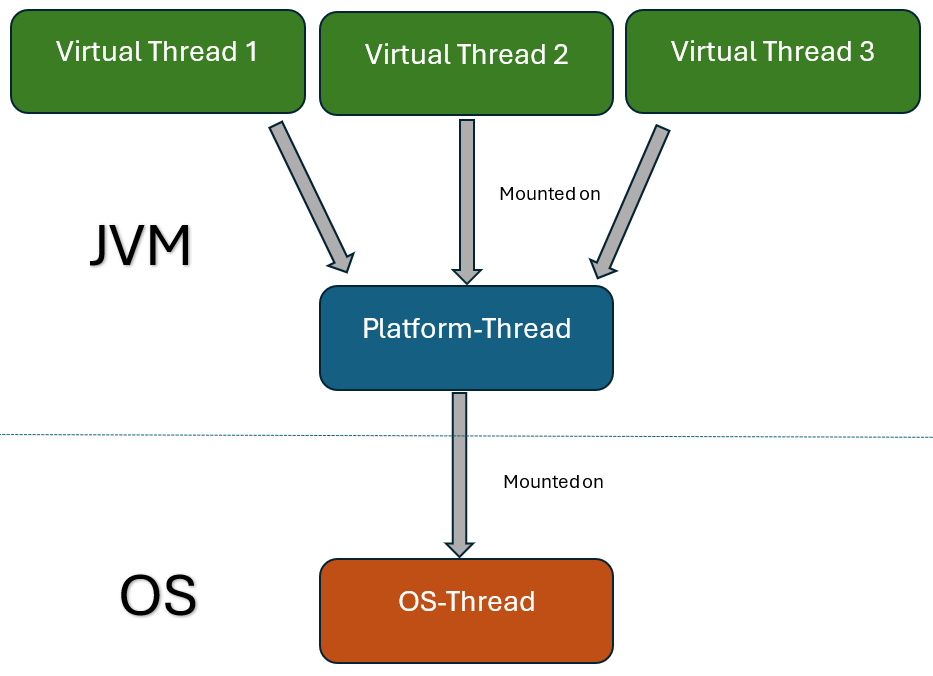
\includegraphics[width=0.6\textwidth]{VTs}
        \caption{Virtuelle Threads in der JVM}
        \label{fig:VTs}
    \end{figure}

    Da \Glspl{vt} vollkommen von der \gls{jvm} verwaltet werden und diese über die Art von Aufgabe und derzeitigen Zustand des Threads Bescheid weiß, kann die
    \gls{jvm} einen \gls{vt} von dem ihm zugeteilten \gls{pt} temporär lösen und einen anderen \gls{vt} darauf Code ausführen lassen, da das Blockieren von \Glspl{vt}
    sehr billig ist. Dies hat zur Folge, dass \Glspl{vt} nur dann Rechenzeit erhalten, wenn sie auch benötigt wird. Somit wird der Durchsatz an Recheninstruktionen
    eines \gls{pt} stark erhöht.
    Wird aber nur ein einzelner Thread benötigt, können diese Vorteile nicht genutzt werden. Der \gls{pt}, dem der \gls{vt} zugewiesen wurde, bindet den \gls{ot} auch
    an sich, selbst wenn kein \gls{vt} Code ausführt.
    \cite{JEP444}

    \begin{figure}[H]
        \centering
        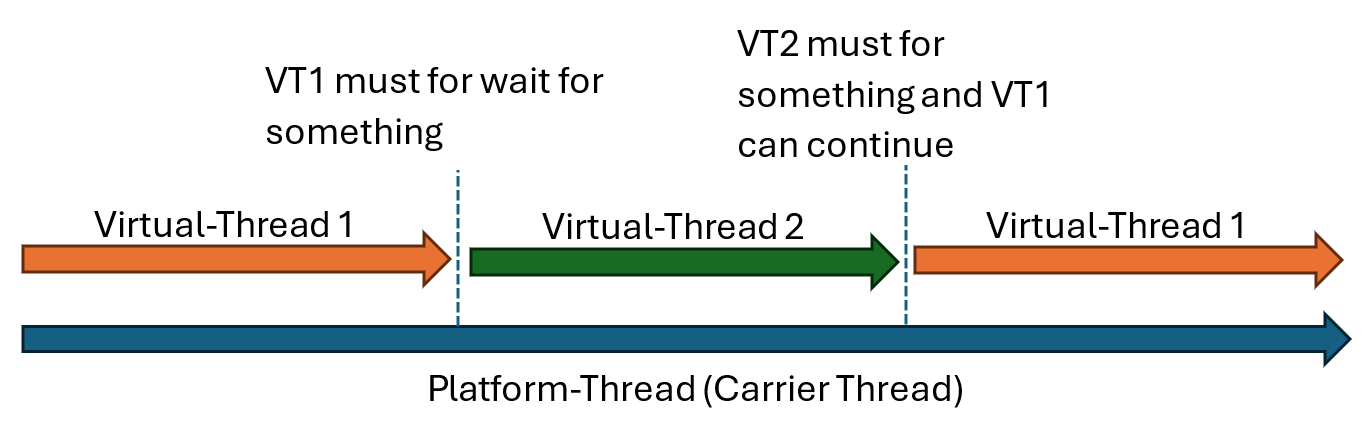
\includegraphics[width=0.67\textwidth]{VT_Coroutine}
        \caption{Coroutine von \Glspl{vt}}
        \label{fig:VT_Coroutine}
    \end{figure}

    Die \gls{jvm} kann auch die initiale Ressourcenzuweisung bei \Glspl{vt} viel präziser durchführen als das Betriebssystem bei \Glspl{ot} die mit jedem neuen \gls{pt}
    erstellt werden. Durch die enge Bindung eines \GLSpl{pt} an seinen \gls{ot} wird der Speicher für den Stack bei der Erstellung des Threads festgelegt.
    Eine dynamische Veränderung der Größe wird nicht unterstützt. Übersteigt die benötigte Größe des Stacks den Vorgaben der \gls{jvm}, wird ein \texttt{StackOverflowError}
    geworfen \cite{jvmSpecification}. Diese initiale Größe kann mit der Option \texttt{-Xss"gewünschte Größe"} für die Ausführung der \gls{jvm} verändert werden wobei 
    je nach Betriebssystem und \gls{jvm} auch hier Einschränkungen gelten oder im Konstruktor des Threads mitgegeben werden.
    Da das Betriebssystem nicht weiß wie spezifische Programmiersprachen ihren Stack verwalten, allokiert
    es den Speicher für den Stack eher großzügig \cite{ProjectLoom}.
    \Glspl{vt} hingegen speichern ihren Stack als \texttt{stack chunk object} im Heap ab. Diese können zur Laufzeit wegen ihrer losen Bindung zu \Glspl{ot},
    dynamisch ihre Größe ändern. 
    Im Gegensatz zu \Glspl{pt} sind \Glspl{vt} auch keine "GC-roots", also Startobjekte für den Speicherfreigabe-Prozess. Alle nicht durch GC-roots erreichbaren
    Objekte werden vom "Garbage Collector" freigegeben. Dadurch werden die in \Glspl{vt} enthaltenen
    Referenzen nicht immer vom Garbage Collector durchwandert. Wird beispielsweise ein \gls{vt} durch ein \texttt{BlockingQueue.take} blockiert und kein anderer Thread eine
    Referenz auf den \gls{vt} oder die \texttt{BlockingQueue} besitzt, wird der \gls{vt} freigegeben. Dies ist erwünschtes Verhalten, da dieser in diesem Fall 
    nicht wieder entblockt werden kann. Würde das nicht passieren spräche man von einem "Thread-Leck", einem Thread der nutzlos im Hintergrund ausgeführt wird und somit
    Systemressourcen verschwendet. 
    Sollte der \gls{vt} aber laufen oder ein anderer Thread eine Referenz auf die \texttt{BlockingQueue} enthalten ist der 
    \gls{vt} über die GC-root des \gls{pt} erreichbar und bleibt bestehen \cite{JEP425}.
    Vor allem bei Anwendungen, die viele Threads über einen längeren Zeitraum  laufen lassen, trägt das Verhalten von \GLSpl{vt} zur Effizienz und Stabilität bei.
    Ansonsten unterscheiden sich \Glspl{vt} nicht stark von \Glspl{pt} und werden von den gleichen Problemen geplagt wie beispielsweise Deadlocks, Race Conditions\cite{JEP425}.
% Thread leaks + warum sie bei vts weniger häufig auftreten und warum ewig blockierte vts nicht ganz so schlimm sind 

\subsection{Wie werden VTs benutzt?}
\label{subsec:WieWerdenVTsBenutzt?}

    Die Erstellung und Verwendung von virtuellen Threads unterscheidet sich nicht stark von den Platform-Threads. 
    \begin{program} [H]
        \caption{Erstellung eines \Glspl{vt}}
        \label{prog:ErstellungEinesVT}
    \begin{JavaCode}[language=Java, numbers=left]
public static void main(String[] args) {
    Thread vt = Thread.ofVirtual().name("VirtualThread").unstarted(() -> {
        System.out.println("Hello from a virtual thread!");
    });
    vt.setPriority(Thread.MAX_PRIORITY);
    vt.start();
    Thread vt1 = Thread.startVirtualThread(() -> {
        System.out.println("Hello from another virtual thread!");
    });
    try {
        vt.join(); vt1.join();
    } catch (InterruptedException e) {
        e.printStackTrace();
    }
}\end{JavaCode}
    \end{program}
    Anstatt \texttt{new Thread(Runnable task).start();} wird der Ausdruck aus Zeile 2 in Programm 
    \ref{prog:ErstellungEinesVT} benutzt um einen neuen Thread zu erstellen. Dabei kann der \texttt{unstarted} Methode ein \texttt{Runnable} mitgegeben werden um den Thread später mit \texttt{start} zu starten. Alternativ kann auch ohne der 
    \texttt{unStarted} Methode \texttt{.start(Runnable r)} aufgerufen werden um den Thread sofort zu starten. Sollte ein \gls{vt} sofort gestartet werden, kann auch \texttt{startVirtualThread} wie in Zeile 9 benutzt werden. Diese Methode nimmt ebenfalls ein
    \texttt{Runnable} als Parameter. \texttt{Thread.join()} lässt genauso wie bei \Glspl{pt} den aktuellen Thread 
    auf die Beendung des Threads warten, für den \texttt{.join()} aufgerufen wurde. Die Nachteile dieser Art der Verwendung sind Codeduplizierung und erhöhter Aufwand
    beim Starten mehrerer Threads, da Eigenschaften wie der Name für jeden Thread individuell angepasst werden müssen. Typische Anwendungsfälle sind schnelle
    einmalige Aufgaben, die sofort und ohne große Konfiguration ausgeführt werden sollen \cite{oracle21Thread}.
    % beispiel für einen Vt mit return wert über eine FutureTask<>

    \begin{program} [H]
        \caption{\Glspl{vt} mit Rückgabewert}
        \label{prog:VTMitRückgabewert}
    \begin{JavaCode}[language=Java, numbers=left]
public static void main(String[] args) {
    FutureTask<String> futureTask = new FutureTask<>(() -> {
        Thread.sleep(1000);
        return "Task completed";
    });
    Thread.ofVirtual().start(futureTask);
    try {
        System.out.println(STR."Result: \{futureTask.get()}");
    } catch (Exception e) {
        e.printStackTrace();
    }
}\end{JavaCode}
    \end{program}
    Sollte der auszuführende Code eine Rückgabewert liefern kann wie in \ref{prog:VTMitRückgabewert} in Zeile 6 dem Thread eine \texttt{FutureTask<>} mitgegeben werden. Diese nimmt wiederum
    ein \texttt{Callable<>} das im Gegensatz zum \texttt{Runnable} einen Wert returniert. Das Ergebnis kann wie in Zeile 8 mit der Methode \texttt{get()} abgefragt werden.
    Diese Methode wartet auf das Ergebnis indem sie den Eltern-Thread blockiert und ersetzt somit das \texttt{join()}.



    Weiters besteht auch die Möglichkeit einen \texttt{Thread.Builder} zu benutzen, der die Anpassung solcher Eigenschaften wie eine Zeichenkette und fortlaufende Zahl
    als Name selbständig weiterführt.
    Bei \Glspl{pt} verändert \texttt{.setPriority(int)} je nach Betriebsystem und Implementierung der \gls{jvm} die Priorität des Threads im Prozess-Scheduler. Bei \Glspl{vt} ist dieser Methodenaufruf in Java 21 zwar
    möglich, hat aber keine Auswirkungen da die Priorität auf \texttt{NORM\_PRIORITY} fixiert wurde. Dies könnte sich aber in zukünftigen Versionen ändern \cite{JEP444}.

    
    
    \begin{program} [H]
        \caption{Beispiel eines \texttt{Thread.Builder.OfVirtual} in Java}
        \label{prog:ErstellungEinesVTBuilders}
    \begin{JavaCode}[language=Java, numbers=left]
public static void main(String[] args) {
    try {
        Thread.Builder builder = Thread.ofVirtual().name("worker-", 0);
        Runnable task = () -> {
            // do something
        };
        // name "worker-0"
        Thread t1 = builder.unstarted(task);
        t1.setPriority(Thread.MAX_PRIORITY);    //Priority is set for each Thread 
                                                //individually   
        t1.start(); t1.join();
        System.out.println(t1.getName() + " terminated");
        // name "worker-1"
        Thread t2 = builder.start(task);   
        t2.join();  
        System.out.println(t2.getName() + " terminated");
    } catch (InterruptedException e) {
        e.printStackTrace();
    }
}\end{JavaCode}
    \end{program}

    Dabei können Regeln für verschiedene Attribute wie eine Namenskonvention
    in einem Schritt für alle späteren Threads festgelegt werden, was Codeduplizierung entgegenwirkt.
    Die Methode \texttt{name(String, long)} ermöglicht eine automatisierte fortlaufende Benennung zukünftig erstellten Threads. Wie wie in Zeile 3 in Programm 
    \ref{prog:ErstellungEinesVTBuilders} zu sehen nimmt die Methode einen Präfix in Form einer Zeichenkette und einen Startwert vom primitiven
    Datentypen \texttt{long}. Der erste durch den Builder erstellte Thread als Namen eine Konkatinierung des Präfixes und des Startwertes. Bei jedem weiteren Thread wird der Startwert um eins inkrementiert. Lässt man den Startwert als Methodenparameter weg, heißen alle Threads gleich 
    \cite{oracle22Builder}. 

    \begin{program} [H]
        \caption{Example of a virtual threadexecutor in Java}
        \label{prog:ErstellungEinesExecutors}
    \begin{JavaCode}[language=Java, numbers=left]
public static void main(String[] args) {
    try (var executor = Executors.newVirtualThreadPerTaskExecutor()){
        IntStream.range(0, 1000).forEach(i -> {
            executor.execute(() -> {     //.submit() returns a Future<> object that can be used to retrieve the result of a computation; .execute() does not return a result.
                System.out.println("Thread " + i + " started");
            });
        });
    }       // executor.close() is called is called implicitly and the Thread waits for all tasks to finish
    System.out.println("All Tasks finished"); 
}\end{JavaCode}
    \end{program}

    Wird eine große Anzahl an \Glspl{vt} benötigt,  ist ein Executor bzw. Threadpool empfehlenswert. Dieser sollte in Kombination mit einem
    try-with-resources-Block verwendet werden, da dieser beim Verlassen des Blockes implizit geschlossen wird. Wird dies nämlich nicht gemacht kann es
    im Falle einer Ausnahme dazu kommen dass ein Thread nicht beendet wird und so als Thread-Leck weiterhin im Hintergrund Systemressourcen verschwendet.
    Der \texttt{.newVirtualThreadPerTaskExecutor()}
    erstellt im Gegensatz zum \texttt{.newFixedThreadPool()} für jede Aufgabe einen neuen \gls{vt}.
    Sollten die Aufgaben einen Wert retournieren muss anstatt \texttt{execute} die Methode \texttt{submit} benutzt werden. Dies retourniert ein \texttt{Future<T>}Objekt 
    \cite{oracle21VritualThreads}.
    Der von der \texttt{Future} enthaltene Wert kann mit der
    \texttt{get}  Methode ausgelesen werden. Dabei handelt es sich um eine blockierende Instruktion. Daher wird die Ausführung des Eltern-Threads bis zur
    Beendung des Kind-Threads angehalten \cite{oracle21Future}.
    


\section{Structured Concurrency}                                 % 4 Seiten ---------------------------------------------------------------------------------------------------------
\label{sec:Structured Concurrency}

    Structured Concurrency (strukturierte Nebenläufigkeit) ist ein Programmierkonzept, das darauf abzielt, die Handhabung von nebenläufigen Aufgaben zu vereinfachen und sicherer zu machen.
    Es stellt sicher, dass alle gestarteten Aufgaben innerhalb eines bestimmten Bereichs abgeschlossen werden, bevor der Bereich verlassen wird.
    Dies führt zu besser lesbarem und wartbarem Code und reduziert die Wahrscheinlichkeit von Fehlern.

\subsection{Was ist Structured Concurrency?}
\label{subsec:WasistSC?}
    Der Bereich \emph{strukturierte Nebenläufigkeit (Structured Concurrency)} in Project Loom fügt \texttt{\Glspl{sts}} zur Standartbibliothek von Java hinzu
    und befindet sich derzeit noch in
    aktiver Entwicklung. Das heißt, dass sich verschiedene Funktionalitäten ändern oder wieder entfernt werden können.
    Die zu strukturierten Nebenläufigkeit gehörigen Klassen ermöglichen
    es, eine Gruppe von parallelen Teilaufgaben als eine Einheit zu koordinieren. Allgemeine Ausführungslogik und Fehlerbehandlung kann dadurch schon vorher festgelegt und 
    wiederverwendet werden.
    Wie der Name bereits verrät, wird dabei ein Block festgelegt, in dem diese Teilaufgaben erstellt und behandelt werden.
    Dadurch müssen die Teilaufgaben vor dem Hauptprozess, in dem sie gestartet wurden, beendet werden.
    \cite{oracle21SC}

    \begin{program} [H]
        \caption{Beispiel für einen einfachen \gls{sts}}
        \label{prog:BeispielFürEinenEinfachenSts}
    \begin{JavaCode}[language=Java, numbers=left]
public static void main(String[] args) {
    try (var scope = new StructuredTaskScope<>()) {
        StructuredTaskScope.Subtask<String> result1 = scope.fork(() -> {
            Thread.sleep(1000);
            return "Result from task 1";
        });
        var result2 = scope.fork(() -> {
            Thread.sleep(2000);
            throw new RuntimeException("Task 2 failed");
        });
        StructuredTaskScope.Subtask<Integer> result3 = scope.fork(() -> {
            Thread.sleep(3000);
            return 3;
        });
        scope.join();                        // Waits for all subtasks to complete
        if (result1.state() == StructuredTaskScope.Subtask.State.SUCCESS){
            System.out.println(result1.get());  
        } 
        System.out.println(result2.get());   // Throws an IllegalStateException
        System.out.println(result3.get());
    } catch (Exception e) {                 // calls .close() implizit.
        e.printStackTrace();
    }
}\end{JavaCode}
    \end{program}
    Wird der \gls{sts} ohne Typ erstellt können die einzelnen Teilprozesse Objekte verschiedener Typen returnieren. \texttt{new StructuredTaskScope<Integer>()}
    hätte beispielsweise eine einschränkende Wirkung.
    Es wird stark empfohlen, einen \gls{sts} in Form eines try-with-resources-Blocks zu realisieren, da dieser den Gültigkeitsbereich wieder schließt. In diesem Block
    werden Teilaufgaben mit der Methode \texttt{.fork(Runnable r)} erschaffen. Diese haben den Rückgabewert \texttt{StructuredTaskScope.Subtask<T>}, wobei sie keine
    primitiven Datentypen aufnehmen können. Mit \texttt{.state()} kann überprüft werden, ob die einzelnen Ausführungen erfolgreich waren.
    Wichtig dabei ist der Aufruf von \texttt{.join()}. Dadurch wartet der \gls{sts}, darauf dass entweder alle Teilprozesse beendet werden oder fehlschlagen, oder
    eine andere vordefinierte Abbruchbedingung erreicht wird.
    \cite{oracle21STS}

    \begin{program} [H]
        \caption{Beispiel für ShutdownOnFailure}
        \label{prog:BeispielFürShutdownOnFailure}
    \begin{JavaCode}[language=Java, numbers=left]
public static void main(String[] args) {
    StructuredTaskScope.Subtask<String> result1 = null;
    StructuredTaskScope.Subtask<String> result2 = null;
    StructuredTaskScope.Subtask<String> result3 = null;
    try (var scope = new StructuredTaskScope.ShutdownOnFailure()) {            // shuts down the scope if a subtask fails
        result1 = scope.fork(() -> {
            Thread.sleep(1000);
            return "Result from task 1";
        });
        result2 = scope.fork(() -> {         // used to return a Future<> object
            Thread.sleep(2000);
            throw new RuntimeException("Task 2 failed");
        });
        result3 = scope.fork(() -> {
            Thread.sleep(5000);
            return "Result from task 3";
        });
        scope.join().throwIfFailed();
    } catch (Exception e) {
        System.out.println("Scope failed");
    }
    System.out.println(result1.get());                                          
    System.out.println(result2.get());         //Throws an IllegalStateException
    System.out.println(result3.get());        // Throws an IllegalStateException due to the exception in the second task
}\end{JavaCode}
    \end{program}
    Eine der zwei abgeleiteten verschachtelten Unterklassen ist \texttt{ShutdownOnFailure}. Sie ist mit \texttt{final} markiert und steht damit nicht für weitere
    Vererbung zur Verfügung. Der Hauptunterschied zur Basisklasse besteht darin, dass die Ausführung aller Teilprozesse beendet wird, sobald nur einer davon fehlschlägt.
    Dies hat zur Folge, dass alle noch nicht beendeten Aufgaben ebenfalls fehlschlagen und deren Ergebnisse nicht abgefragt werden dürfen. Dieses Verhalten ist besonders dann
    erwünscht wenn alle Teilergebnisse essentiell sind und das Fehlschlagen eines einzelnen Teilprozesses somit das Gesamtergebnis unbrauchbar macht. 

    \begin{program} [H]
        \caption{Beispiel für ShutdownOnSuccess}
        \label{prog:BeispielFürShutdownSuccess}
    \begin{JavaCode}[language=Java, numbers=left]
public static void main(String[] args) {
    StructuredTaskScope.Subtask<String> result1 = null;
    StructuredTaskScope.Subtask<String> result2 = null;
    String result = null;
    try (var scope = new StructuredTaskScope.ShutdownOnSuccess<String>()) {                 // shuts down the scope if a subtask succeeds
        result1 = scope.fork(() -> {
            Thread.sleep(2000);
            return "Result from task 1";
        });
        result2 = scope.fork(() -> {
            return "Result from task 2";
        });
        result = scope.join().result();      // .result() returns the result of the scope
    } catch (Exception e) {
        System.out.println("Scope failed");
        e.printStackTrace();
    }
    System.out.println(result1.get());            // Throws an IllegalStateException because the scope is shut down due to the success of the second task
    System.out.println(result2.get());
    System.out.println(result);
}\end{JavaCode}
    \end{program}
    Die zweite abgeleitete verschachtelte Unterklasse ist \texttt{ShutdownOnSuccess} und ist ebenfalls \texttt{final}. Hierbei werden die Ausführungen gestoppt, falls
    einen Teilaufgabe erfolgreich beendet wird. Eine Abfrage der Ergebnisse der Teilaufgaben ist möglich, wird aber nicht empfohlen, da es nur ein gültiges
    Ergebnis geben kann
    und dieses mit \texttt{.result()} direkt abgefragt werden kann. Dabei wird das Ergebnis direkt zurückgegeben und nicht als \texttt{StructuredTaskScope.Subtask<>}.
    Schlagen alle Teilaufgaben fehl, wird null retourniert.


    % Zitate!!!!!!!!!!!!!!!!!!!!!!!!!

\subsection{Erstellung eines eigenen \texttt{StructuredTaskScopes}}
\label{subsec:ErstellungEinesEigenenSts?}

    Nicht immer erfüllen die zwei Subklassen \texttt{ShutdownOnFailure} und \texttt{ShutdownOnSuccess} den individuellen Anforderungen des Anwenders.
    Es könnte zum Beispiel nur das Kleinste Ergebnis aller erfolgreich abgeschlossenen Aufgaben gewünscht werden oder man möchte alle Ergebnisse mit
    einem Methodenaufruf erhalten ohne sich die \texttt{Subtask<>}s abspeichern zu müssen.
    Die Klasse \texttt{StructuredTaskScopes<T>} wurde nicht mit final markiert und lässt somit Ableitungen zu. Die für die Erstellung individueller Implementierungen wichtigen
    Methoden wurden mit der Sichtbarkeit \texttt{protected} versehen und lassen sich daher nach belieben überschreiben.


    \begin{program} [H]
        \caption{Beispiel für den Aufbau von \texttt{SmallestScope<T>}}
        \label{prog:BeispielFürSmallestScope}
    \begin{JavaCode}[language=Java, numbers=left]
public class SmallestScope<T> extends StructuredTaskScope<T> {
    private final Collection<T> results = new ConcurrentLinkedDeque<>();
    private final Collection<Throwable> exceptions = new ConcurrentLinkedDeque<>();
    private final Comparator<T> comparator;

    public SmallestScope(Comparator<T> comparator) {
        this.comparator = Objects.requireNonNull(comparator);
    }

    @Override
    protected void handleComplete(Subtask<? extends T> subtask) {...}

    public Exception exceptions() {...}

    public T smallest() throws Exception {...}

    @Override
    public SmallestScope<T> join() throws InterruptedException {
        super.join();
        return this;
    }

    @Override
    public SmallestScope<T> joinUntil(Instant deadline)
        throws InterruptedException, TimeoutException{
            super.joinUntil(deadline);
            return this;
    } 
}\end{JavaCode}
    \end{program}
    
    Ein Beispiel für einen individualisierten \gls{sts} ist \texttt{SmallestScope<T>}. Dieser soll nach Beendung oder Fehlschlag aller Teilprozesse das Kleinste 
    aller Ergebnisse liefern.
    Dafür muss zunächst von von \texttt{StructuredTaskScope<T>} abgeleitet werden. Außerdem werden noch zusätzliche Datenkomponenten benötigt wie in den Zeilen 2 bis 4 in
    \ref{prog:BeispielFürSmallestScope} zu sehen ist. 
    Um die einzelnen Teilergebnisse für die weitere Verarbeitung zu speichern wird ein Behälter benötigt.
    Dieser sollte theadsicher sein da mehrere Prozesse darauf zugreifen müssen.
    Da der Benutzer an den Fehlermeldungen der Subprozesse interessiert sein könnte sollten diese ebenfalls in einem threadsicheren Behälter aufbewahrt werden. 
    Um das kleinste Ergebnis ermitteln zu können wird zunächst eine Vergleichsmöglichkeit in Form eines \texttt{Comperator<T>}-Objekts benötigt. Dieses wird über den
    Konstruktor injiziert.
    Das Überschreiben der Methoden \texttt{join()} und \texttt{joinUntil(Instant deadline)} ist nicht essentiell um die Klasse benutzen zu können sondern ermöglicht
    lediglich Methodenverkettung zu ermöglichen. Dies ist zwar nicht dringend nötig wird aber stellt für viele ein erwartetes verhalten dar.

    \begin{program} [H]
        \caption{Überschreiben von \texttt{handleComplete}}
        \label{prog:ÜberschreibenVonHandleComplete}
    \begin{JavaCode}[language=Java, numbers=left]
@Override
protected void handleComplete(Subtask<? extends T> subtask) {
    switch (subtask.state()) {
        case SUCCESS -> results.add(subtask.get());
        case FAILED, UNAVAILABLE -> {
            exceptions.add(subtask.exception());
        }
    }
}\end{JavaCode}
    \end{program}
    Die Methode \texttt{handleComplete()} wird von jedem Thread bei Beendung seiner Aufgabe aufgerufen, vorausgesetzt der \gls{sts} wurde durch z.B. der Methode 
    \texttt{shutdown()} noch nicht beendet.
    Um den gewünschten Effect zu erzielen muss zunächst der Zustand des \texttt{Subtask}s abzufragen. Beim Zustand \texttt{SUCCESS} kann das Ergebnis in den Behälter für Ergebnisse
    gespeichert werden. Ist der Zustand \texttt{FAILED} oder \texttt{UNAVAILABLE} wird die Fehlermeldung abgefragt und in dem dafür vorgesehenen Behälter platziert.

    \begin{program} [H]
        \caption{Returnieren des kleinsten Ergebnisses}
        \label{prog:ReturnierenDesKleinstenErgebnisses}
    \begin{JavaCode}[language=Java, numbers=left]
public T smallest() throws Exception {
return results.stream()
        .filter(Objects::nonNull)
        .min(comparator)
        .orElseThrow(this::exceptions);
}\end{JavaCode}
    \end{program}
    Um das kleinste Ergebnis später ermitteln und abfragen zu können wird einen neue Methode \texttt{smallest()} benötigt die nach \texttt{join()} oder
    \texttt{joinUntil(instant)} aufgerufen werden kann und das Ergebnis returniert. Dazu wird in dem Behälter mithilfe des Comperators das kleinste Element gesucht
    und zurückgegeben. Dazu wird Javas Stream-API benutzt wobei Objekte deren Wert \texttt{null} beträgt herausgefiltert werden. Sollte dies aus verschiedenen Gründen nicht möglich sein werden alle gesammelten Fehlermeldungen geworfen. 
    \begin{program} [H]
        \caption{Returnieren der Fehlermeldungen}
        \label{prog:ReturnierenDerFehlermeldungen}
    \begin{JavaCode}[language=Java, numbers=left]
public Exception exceptions() {
    Exception exception = new Exception();
    this.exceptions.forEach(exception::addSuppressed);
    return exception;
}\end{JavaCode}
    \end{program}
    Um den Nutzenden zu ermöglichen, die Fehlermeldungen der fehlgeschlagenen Teilprozesse zu erhalten wird \gls{sts} um die Methode \texttt{exceptions()} erweitert.
    Diese returniert eine neue Fehlermeldung der alle Fehlermeldungen aus dem Behälter aus \ref{prog:BeispielFürSmallestScope} in Zeile 3 angehängt werden.

    \begin{program} [H]
        \caption{Beispiel für die Verwendung von \texttt{SmallestScope<T>}}
        \label{prog:VerwendungVonSmallestScope}
    \begin{JavaCode}[language=Java, numbers=left]
public static void scopesSmallest() {
    StructuredTaskScope.Subtask<Integer> result1 = null;
    Integer result = null;

    try (var scope = new SmallestScope<Integer>(Integer::compareTo)) {                                         
        result1 = scope.fork(() -> { 
            Thread.sleep(1000); 
            return 4; 
        });
        scope.fork(() -> { throw new RuntimeException("Task 2 failed"); });
        scope.fork(() -> { 
            Thread.sleep(2000); 
            return 3; 
        });

        result = scope.join().smallest();
        if (result1.state() == StructuredTaskScope.Subtask.State.SUCCESS) {
            System.out.println(STR."result from the 1st Thread: \{result1.get()}");
        }
        scope.exceptions().printStackTrace();
    } catch (Exception e) {
        e.printStackTrace();
    }
    System.out.println(STR."smallest result: \{result}");
}\end{JavaCode}
    \end{program}
    Wie in \ref{prog:BeispielFürSmallestScope} ersichtlich ist kann \texttt{SmallestScope} nun ähnlich wie die anderen \Glspl{sts} benutzt werden. Der Konstruktor benötigt
    aber einen Komparator, hier \texttt{Integer::compareTo} in Zeile 5, als Parameter. Teilergebnisse der einzelnen Prozesse können ebenfalls wieder abgefragt werden. Diese Abfragen
    bringen dieselben bereits besprochenen Probleme mit sich. Die einzelnen Teilprozesse müssen 
    aber auch wie bei \texttt{ShutdownOnSuccess} den gleichen Typen returnieren wie im Generika festgelegt. Da die Methode \texttt{join()} dementsprechend überschrieben
    wurde, kann die Ergebnisabfrage \texttt{smallest()} an diese gekettet werden. Für Debugging-Zwecke können alle Fehlermeldungen wie in Zeile 20 mit \texttt{exceptions()}
    erhalten werden. Sollten alle Teilprozesse fehlschlagen werden diese aber ebenfalls geworfen. 

\section{Scoped Values}                                 % 3 Seiten ---------------------------------------------------------------------------------------------------------
\label{sec:Scoped Values}
    
    Scoped Values (Bereichsgebundene Werte) sind ebenfalls Teil von Projekt Loom und eine neue Funktion in der \gls{jvm}, die es ermöglicht,
    Werte sicher und effizient innerhalb eines bestimmten Bereichs zu teilen.
    Sie bieten eine Alternative zu ThreadLocal-Variablen und sind besonders nützlich in Umgebungen mit vielen \Glspl{vt}. 
    Scoped Values verbessern die Lesbarkeit und Wartbarkeit des Codes, indem sie die Lebensdauer und Sichtbarkeit von Werten klar definieren.
    
\subsection{Was sind Scoped Values?}
\label{subsec:WasSindSV?}
    Bereichsgebundene Variablen ermöglichen es Werte bzw. Variablen in Bereichen oder Methoden sichtbar zu werden. 
    Die damit assoziierte Klasse \texttt{ScopedValue<>} stellt dabei ein sogenanntes Wrapper- oder Speicherobjekt dar, das dem tatsächlichen Datenwert und den Zugriff darauf verwaltet.
    Dabei wird der Wert auch in allen Methoden die in diesem Gültigkeitsbereich direkt oder indirekt aufgerufen wurden verfügbar ohne die Nutzung von Methodenparametern.
    Somit ist ein \texttt{ScopedValue} ein impliziter Methodenparameter entlang der Sequenz aufgerufener Methoden der nicht manuell definiert werden muss.
    Dieses Verhalten tritt nicht nur für den derzeitigen Thread auf sondern auch für alle darin erzeugten Kind-Threads.
    So können zum Beispiel in Frameworks Abhängigkeiten verfügbar gemacht werden ohne sie explizit durch Methodenschnittstellen reichen zu müssen \cite{JEP481}. 
    \begin{program} [H]
        \caption{Beispiel für die Verwendung von \texttt{ScopedValue<>}}
        \label{prog:VerwendungVonSV}
    \begin{JavaCode}[language=Java, numbers=left]
public class ScopedValueExample {
    private static final ScopedValue<String> someName = ScopedValue.newInstance();
    private static final ScopedValue<String> someName2 = ScopedValue.newInstance();

    public static void main(String[] args) {
        ScopedValue.Carrier carrier = ScopedValue.where(someName, "Alice");
        carrier.where(someName2, "Herbert").run(()->{
            System.out.println(STR."Name: \{someName2.get()}");
            printName();
            ScopedValue.where(someName, "Bob").run(ScopedValueExample::printName);
            System.out.println(STR."Name: \{someName.get()}");
        });
        if (someName.isBound()) {
            System.out.println(STR."Name: \{someName.get()}");
        } else {
            System.out.println(STR."someName is not bound");
        }
    }

    private static void printName() {
        System.out.println(STR."Name: \{someName.get()}");
    }
}\end{JavaCode}
    \end{program}   
    Wie in \ref{prog:VerwendungVonSV} in Zeile 2 demonstriert, muss eine neue Instanz mithilfe der statischen Fabrikmethode \texttt{newInstance()} erstellt werden da der Konstruktor als privat 
    markiert wurde. 
    Die statische Methode \texttt{where(ScopedValue<T>, T)} bindet einen Wert an eine bereichsgebundene Variable und gibt ein Objekt der Klasse \texttt{ScopedValue.Carrier} zurück.
    Dieses Objekt verwaltet die \texttt{ScopedValue}s und deren Werte und Gültigkeitsbereiche. Werden weitere Wertbindungen benötigt kann auf dieses Objekt wiederum die \texttt{where} Methode 
    aufgerufen werden. Dieser Aufruf modifiziert aber nicht das Original sondern returniert ein neues Objekt mit allen alten und neuen Einträgen. Der Bereich kann als \texttt{Runnable}
    der Methode \texttt{run(Runnable)} mitgegeben werden \cite{oracle22Carrier}. 
    Die Methode \texttt{isBound()} returniert "wahr" sollte sich deren Aufruf in einem Bereich befinden wo ein gültiger Wert gebunden wurde was in Zeile 13 nicht der Fall ist.
    Sollte der Methodenaufruf in Zeile 10 ohne solche Überprüfung erfolgen, würde zur Laufzeit eine \texttt{NoSuchElementException} geworfen werden.
    Die Zeilen 10 und 11 zeigen dass eine Verschachtlung der der Wertebereiche einer Variable auch möglich ist. Der Ausdruck in Zeile 10 überschreibt den in Zeile 6 definierten Wert für die Variable
    \texttt{someValue} für einen Bereich in dem die Methode \texttt{printName} aufgerufen wird. Da dieser Gültigkeitsbereich in Zeile 11 wieder erlöschen ist returniert der Aufruf
    \texttt{someName.get()} wieder den Wert des äußeren Bereichs. Vererbung zwischen Threads ist nur bei Strukturierter Nebenläufigkeit (Structured Concurrency) möglich. Die Bindungen der Werte
    werden dabei nur für Threads übernommen die mit der \texttt{fork()}-Methode gestartet werden.
    \begin{program} [H]
        \caption{Beispiel für Vererbung bei \texttt{ScopedValue<>}}
        \label{prog:VererbungBeiSV}
    \begin{JavaCode}[language=Java, numbers=left]
private static final ScopedValue<String> NAME = ScopedValue.newInstance();
ScopedValue.runWhere(NAME, "duke", () -> {
    try (var scope = new StructuredTaskScope<String>()) {
        scope.fork(() -> {System.out.println(STR."Name: \{NAME.get()}");return null;});
    }
    Thread.ofVirtual().start(() -> {
        System.out.println(STR."Name: \{NAME.get()}");
    });    
});\end{JavaCode}
\end{program}
In Programm \ref{prog:VererbungBeiSV} ist die die Abfrage des Wertes in Zeile 4 problemlos möglich. Die Abfrage in Zeile 7 wirft
jedoch eine \texttt{IllegalStateException} in Thread die nicht in \Glspl{sts}
erstellt wurden keine Vererbung stattfindet.

\subsection{Unterschiede ScopedValues und ThreadLocal}
\label{subsec:UnterschiedeScopedValuesundThreadLocal}

    Es war nie das Ziel von \texttt{ScopedValues}, \texttt{ThreadLocal} vollends zu ersetzen. Vielmehr sollte eine Alternative mit Vorteilen in spezifischen Situationen geschaffen werden.
    Jeder \gls{pt} hat eine Instanz von \texttt{ThreadLocal.ThreadLocalMap} als Datenkomponente. Dieser Datenbehälter ist ein dynamisch wachsendes Feld aus
    der Klasse \texttt{Entry} die eine Referenz auf die \texttt{ThreadLocal}-Klasse als Schlüssel
    und deren für diesen Thread gültigen Wert als Paar abspeichert. Dadurch hat jeder Thread seine eigene Instanz der Variable zur Verfügung stehen, die jederzeit gelesen und beschrieben werden kann.
    Dieser Behälter wird aber nicht vom Thread sondern von der Klasse \texttt{Threadlocal} verwaltet. 
    \begin{figure}[H]
        \centering
        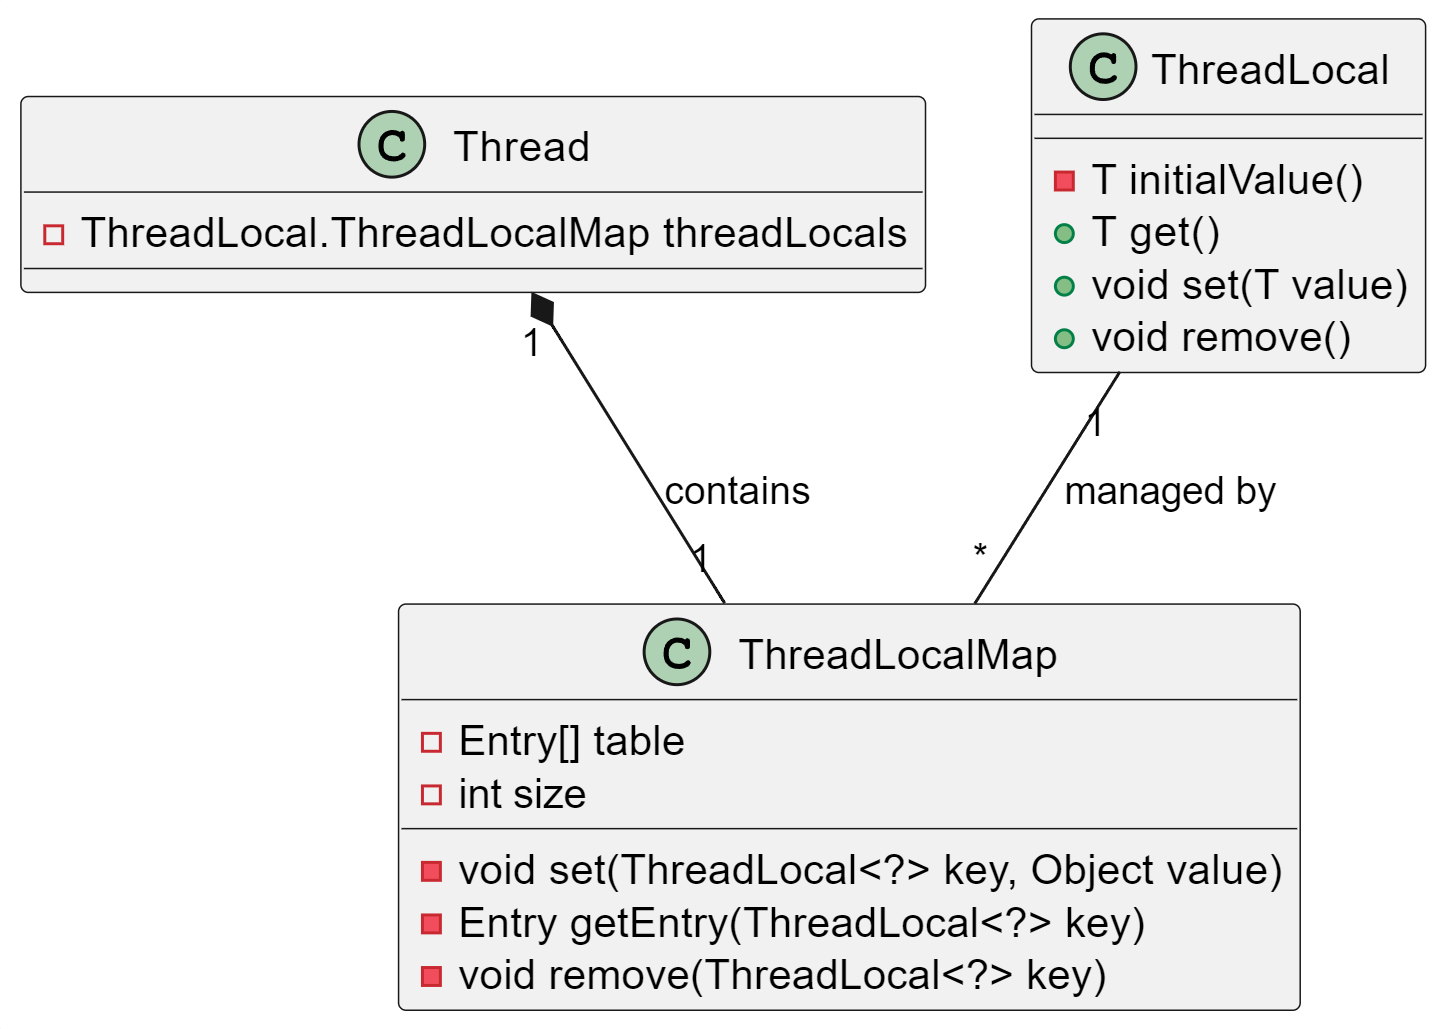
\includegraphics[width=0.6\textwidth]{ThreadLocalUML.png}
        \caption{Überblick Aufbau von ThreadLocal}
        \label{fig:ThreadLocalMap}
    \end{figure}
    Dasselbe gilt auch für \texttt{InheritableTreadLocal}. Wird in einem Thread ein neuer gestartet, erbt dabei aber der Kind-Thread alle Einträge des Eltern-Threads. 
    Ein Vorteil von \Glspl{vt} ist dass sie wegen ihrer Günstigkeit in großen Mengen verfügbar sind und erstellt werden können. Dabei können sich die Eigenschaften von \texttt{ThreadLocal}
    als Problem herausstellen. Vor allem bei großen Variablen kann dies zu einem sehr hohen Speicherverbrauch führen. Bei \texttt{InheritabletreadLocal} kann die Allokation des Speichers
    für die Vererbung zusätzlich einen großen Verwaltungsaufwand bewirken. 

    \texttt{ScopedValue} hingegen ist wie ein Behälter-Objekt das dem tatsächlichen Datenwert und den Zugriff darauf verwaltet. Die Methode \texttt{get()} sucht beim initialen Aufruf nach
    der Wertbindung des innersten Gültigkeitsbereichs. Dabei werden die Ergebnisse in einem in einem kleinen Cache des Threads zwischengespeichert. Dadurch werden nachfolgenden Aufrufe der
    Methode stark beschleunigt. Übersteigt die Menge an bereichsgebundenen Variablen die Größe des Cache, leidet die Geschwindigkeit stark daran. Die Größe beträgt normalerweise 16 Einträge
    und lässt sich mit der \gls{jvm}-Option \texttt{-Djava.lang.ScopedValue.cacheSize=<newSize>} auf eine Größe von 2 bis 16 in 2er-Potenzen verändern. Dabei muss ein Kompromiss
    zwischen Speicherverbrauch und Geschwindigkeit gefunden werden. Werden mehr Werte benötigt kann es sinnvoll sein sie in einem Record zusammenzufassen und so an eine Instanz von ScopedValue
    zu binden. 

    Wie bereits vorher erwähnt ist die Vererbung bei \texttt{TreadLocal} speicher- und laufzeitintensiv da alle Einträge der \texttt{ThreadlocalMap} in den neuen Thread kopiert werden müssen.
    Bei \texttt{ScopedValue} wird dieser Vorgang nicht benötigt. Dadurch fällt sehr viel an Verwaltungsaufwand weg. 

    Bei \texttt{ThreadLocal} wird, wenn einmal mit der \texttt{set}-Methode gesetzt, die Lebensdauer des Wertes nur durch die Lebensdauer des Threads begrenzt und sollte immer mit dem Methodenaufruf
    \texttt{remove} wieder freigegeben werden. Bei langlebigen Threads kann dies zu nicht notwendigen Speicherverbrauch führen. Bei Verwendung eines Threadpools vor allem eines \emph{newCachedThreadPool}
    können bestehende \Glspl{pt}, falls verfügbar, wiederverwendet werden. Diese Vorgehen kann zwar die Geschwindigkeit des Programms erhöhen, jedoch können dadurch auch Variablen,
    wenn nicht manuell entfernt, in eine andere Aufgabe gelangen und so eine potentielle Sicherheitslücke darstellen. Der \emph{Garbage-Collector} kann die Variable nicht freigeben da sie noch über 
    den Thread also einer \emph{GC-root} erreichbar bleibt. Bei \texttt{ScopedValue}s hingegen ist die Lebenszeit an den Gültigkeitsbereich der als \texttt{Runnable} der \texttt{run}-Methode mitgegeben wird,
    gebunden. Dadurch wird der Wert unzugänglich wenn der Gültigkeitsbereich wieder verlassen wird. Eine manuelle Entfernung durch einen Methodenaufruf ist nicht nötig.

    Einen weiteren Unterschied stellt die Veränderbarkeit der Variablen dar. \texttt{ThreadLocal}-Variablen sind uneingeschränkt mit der \texttt{set} Methode veränderbar.
    Auch die Verwendung der Schlüsselwortes \texttt{final} schützt nicht davor. Dadurch wird ein Datenfluss in alle Richtungen zwischen Methoden gewährleistet. Dies kann zu sehr unübersichtlichen 
    Kommunikationsfluss in Form von sogenannten "Spagetti-Code" führen. Die Klasse \texttt{ScopedValue} hingegen lässt einen Datenfluss nur in eine Richtung zu. Der Wert kann innerhalb des 
    Gültigkeitsbereichs durch einen neuen, verschachtelten Gültigkeitsbereich überschrieben werden. Diese Änderung ist aber nicht mehr außerhalb des neuen Bereichs sichtbar und ist damit im Aufrufstapels weiter
    unten nicht gültig \cite{JEP481}.
    \begin{program} [H]
        \caption{ThreadLocal}
        \label{prog:ThreadLocal}
    \begin{JavaCode}[language=Java, numbers=left]
static ThreadLocal<String> threadLokal = new ThreadLocal<>();
public static void main(String[] args) {
    threadLokal.set("the negative side of Threadlocal");
    printHello();
    System.out.println(STR."This is a Methode to show \{threadLokal.get()}");
    threadLokal.remove();
}

public static void printHello() {
    threadLokal.set(Thread.currentThread().toString());
    System.out.println(STR."Hello from \{threadLokal.get()}");
}\end{JavaCode}
    \end{program}
    In \ref{prog:ThreadLocal} in Zeile 3 wird der Wert der thread-lokalen Variable gesetzt. In Zeile 4 wird eine Methode aufgerufen die den Wert aus diversen Gründen überschreibt. Die Wertabfrage in Zeile 5
    returniert den zuletzt gesetzten Wert auch wenn dies in einer anderen Methode geschieht. Das Verhalten von \texttt{ScopedValue} kann in \ref{prog:VerwendungVonSV} observiert werden.








\chapter{Messungen}
\label{cha:Messungen}
    In Rahmen dieser Arbeit wurden verschiedene Messungen und Benchmarks des Laufzeitverhaltens durchgeführt, um Vergleiche zwischen den bereits bekannten Technologien und den Neuerungen in Projekt Loom 
    durchführen zu können. 

\section{Testumgebung}                                         
\label{sec:Testumgebung}

    Alle getesteten Programmen wurden mittels Java Development Kit (JDK) \emph{Eclipse Temurin 22.0.2} kompiliert und ausgeführt. Als JVM-Optionenen wurde 
\begin{verbatim}
--add-exports java.management/sun.management=ALL-UNNAMED 
--add-exports jdk.management/com.sun.management.internal=ALL-UNNAMED 
-XX:+UnlockDiagnosticVMOptions -XX:+DebugNonSafepoints\end{verbatim}
    benutzt.
    Das System nutzt Windows 10 Professional als Betriebssystem und ist mit einem "i7-8086K" Prozessor ausgestattet. Dabei handelt es sich um eine CPU mit x86-64-Anweisungssatz und 6 
    Kernen mit einer Taktfrequenz zwischen 4 und 5 GHz. Als Arbeitsspeicher kamen  16 GB DDR4-RAM zum Einsatz die auf 2600MHz takten. Die integrierte Graphikeinheit der CPU wurde, 
    um eine zusätzliche Wärmebelastung zu vermeiden, deaktiviert. 
    Für die Laufzeitmessungen wurde das "Java Microbenchmark Harness (JMH)" Version 1.37 verwendet.
    Es wurden keine Maßnahmen ergriffen, um hardwarespezifische Einflussfaktoren wie den Taktraten-Boost der CPU zu unterbinden.


\section{Laufzeitmessungen bei Threads in verschiedenen Szenarien}                                         
\label{sec:LaufzeitmessungenbeiThreadsinverschiedenenSzenarien}

    Um die Stärken und Schwächen von \Glspl{vt} im Vergleich zu \Glspl{pt} genauer ermitteln bzw. evaluieren zu können sind Laufzeitmessungen in verschiedenen Szenarien nötig. 
    Anhand dieser Messungen kann ein Leitfaden für die Wahl zwischen \Glspl{pt} und \Glspl{vt} erstellt werden. 
    Folgende Szenarien werden behandelt:
    \begin{itemize}
        \item Laufzeitmessungen unter hoher Auslastung (CPU-intensive Berechnungen),  
        \item Laufzeitmessungen bei sehr vielen Threads und blockierenden (wartenden) Aufgaben.
        \item Laufzeitmessungen bei einer Abhängigkeit zwischen Threads und Verwendung einer geteilten Ressource.
    \end{itemize}


\subsection{Laufzeitmessungen bei Threads unter hoher CPU-Auslastung}                                         
\label{subsec:LaufzeitmessungenbeiThreadsunterhoherAuslastung}

    Ziel der ersten Laufzeitmessung war es herauszufinden wie sich \Glspl{vt} unter ständiger hoher Auslastung schlagen. Die vom Thread ausgeführte Aufgabe greift auf keine 
    externen Ressourcen zu und weist auch keine Abhängigkeiten auf andere Prozesse auf. Die Berechnungen sind daher ohne Unterbrechung durchführbar.
    Dieser Vergleich nutzt dadurch keine der von den Entwicklern erwähnten  Stärken von \Glspl{vt}.
    \begin{program} [H]
        \caption{Benchmark eines \Glspl{vt} unter hoher Auslastung}
        \label{prog:BenchmarkEinesVTUnterHoherAuslastung}
    \begin{JavaCode}[language=Java, numbers=left]
@State(Scope.Benchmark)
public class PerformanceVirtual {

    @Param("10000")
    public int nonsenseIterations;

    @Benchmark
    @BenchmarkMode(Mode.SampleTime)
    @OutputTimeUnit(TimeUnit.MILLISECONDS)
    public void testMethodeVirtual() throws InterruptedException {
        Thread.startVirtualThread(() -> {
            for (int i = 0; i < nonsenseIterations; i++)
                Utility.executeNonesense();
        }).join();
    }
}\end{JavaCode}
    \end{program}
    Dieser Benchmark startet einen \gls{vt} und lässt ihn durchgängige rechenintensive Aufgaben erledigen. Um eine Messung durchführen zu können, wartet der Eltern-Thread auf
    die Beendung der Aufgaben. Um den Unterschied in der Laufzeit sichtbarer zu gestalten und die Auswirkungen externer Störungsfaktoren zu minimieren,
    wird die Berechnung wiederholt ausgeführt. Die Anzahl der Ausführungen ist in Zeile 4 definiert. Der Methodenaufruf \texttt{executeNonesense()} in Zeile 13 stellt die Berechnung dar.
    Die Methode wird in \ref{prog:ExecuteNoneSense} näher erklärt. Der Benchmark für die \gls{pt} ist bis auf die Art des verwendeten Threads ident.
    Als Ergebnis wird die gesamte Dauer der Ausführung geliefert. 

    \begin{program} [H]
        \caption{Rechenintensive Prozedur}
        \label{prog:ExecuteNoneSense}
    \begin{JavaCode}[language=Java, numbers=left]
public static void executeNonesense() {
    int limit = 100000; // Adjust this limit for more or less intensity
    boolean[] isPrime = new boolean[limit + 1];
    for (int i = 2; i <= limit; i++) 
        isPrime[i] = true;
    for (int factor = 2; factor * factor <= limit; factor++) {
        if (isPrime[factor]) {
            for (int j = factor; factor * j <= limit; j++) 
                isPrime[factor * j] = false;
        }
    }
    int primeCount = 0;
    for (int i = 2; i <= limit; i++) {
        if (isPrime[i])
            primeCount++;
    }
}\end{JavaCode}
    \end{program}

    Die Methode \texttt{executeNonesense} in \ref{prog:ExecuteNoneSense} errechnet alle Primzahlen zwischen 2 und einer in Zeile 2 definierten Obergrenze. Anschließend wird 
    auch noch die Anzahl der Primzahlen ermittelt. Das Ergebnis ist komplett irrelevant und wird nach der Berechnung nicht weiterverwendet. Wichtig ist nur, dass es sich um
    eine aufwändige Berechnung handelt.

    \begin{figure}[H]
        \centering
        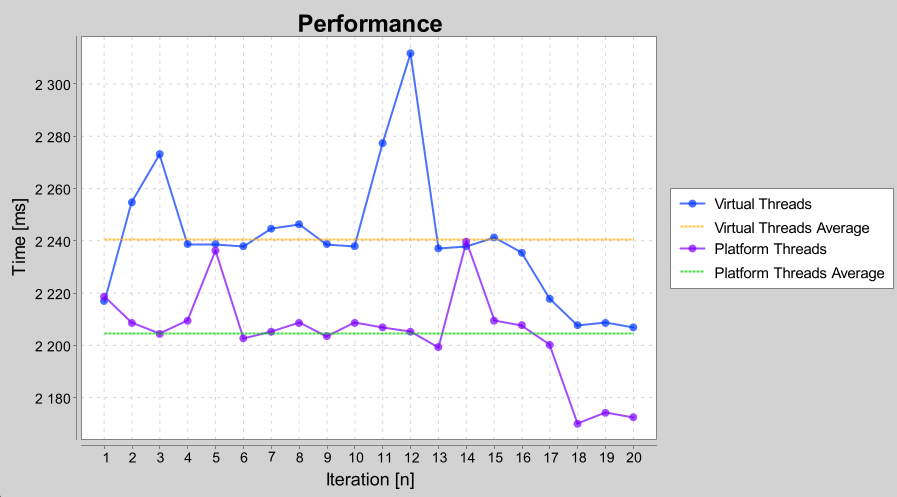
\includegraphics[width=1.0\textwidth]{Performance.png}
        \caption{Laufzeitmessungen bei Threads unter hoher Auslastung}
        \label{fig:Performance}
    \end{figure}

    Die Graphen in Abbildung \ref{fig:Performance} stellen die Ergebnisse dar. Auf der x-Achse sind die einzelnen Messiterationen abgebildet. Die y-Achse ordnet den einzelnen Iterationen die gemessene
    Ausführungsdauer zu.
    Das arithmetische Mittel der Ausführungsdauer der \Glspl{vt} beträgt 2240,6391 Millisekunden (ms). 
    \Glspl{pt} benötigten dafür durchschnittlich 2204,6939 ms. Somit beträgt der mittlere Geschwindigkeitsunterschied 1,6 \% zugunsten der \Glspl{pt}.
    Das Ergebnis ist damit damit begründbar, dass in diesem Fall die von den Entwicklern genannten Verbesserungen der \Glspl{vt} keine Vorteile bieten. Weder die billigere
    Erstellung neuer Instanzen, da wenige Threads gestartet werden, noch Fähigkeit bei blockierenden Aufgaben vom Carrier-Thread gelöst zu werden, da der keine blockierende Aufgaben auftreten und
    auch keine anderen \Glspl{vt} existieren, die diese Rechenzeit beanspruchen könnten. Nur dürfte ein kleiner Overhead existieren der sie im Vergleich zu \Glspl{pt} verlangsamt, da ein \gls{vt} alle seine
    Berechnungen auf einem \gls{pt} ausführt.
    Diese Unterschiede sollten in den meisten Fällen aber vernachlässigbar sein, da die Einbußen sich gering halten und sich solch reine Situationen wie dieser Benchmark in Praxis eher selten 
    ergeben.



\subsection{Laufzeitmessungen bei wartender Auslastung}                                         
\label{subsec:sleep}

    Der nächste Benchmark behandelt einen Fall, bei dem eine hohe Anzahl sehr wenig rechenintensiver Aufgaben parallel gestartet werden. Die Aufgaben selbst simulieren einen blockierenden
    Prozess wie beispielsweise das
    Warten auf die Antwort eines Servers. Die einzelnen Threads werden mittels Executor-Services erstellt. Gegenübergestellt werden ein \texttt{VirtualThreadPerTaskExecutor}, ein \texttt{CachedThreadPool}
    und ein \texttt{ThreadPerTaskExecutor} für \Glspl{pt}. Jeder Thread führt dann ein \texttt{Thread.sleep()} aus und gibt anschließend ein Ergebnis zurück. 
    \begin{program} [H]
        \caption{Laufzeitmessungen bei wartenden Auslastung}
        \label{prog:sleep}
    \begin{JavaCode}[language=Java, numbers=left]
@State(Scope.Benchmark)
public class VirtualThreadSleep {

    @Param("100000")
    public static int iterations;

    @Benchmark
    @BenchmarkMode(Mode.SampleTime)
    @OutputTimeUnit(TimeUnit.MILLISECONDS)
    public static void virtualExecutor() { 
        try (var executor = Executors.newVirtualThreadPerTaskExecutor()) {
            IntStream.range(0, iterations).forEach(i -> {
                Future<Integer> future = executor.submit(() -> {
                    Thread.sleep(Duration.ofSeconds(1)); return i;
                });
            });
        }
    }
}\end{JavaCode}
    \end{program}
    In Programm \ref{prog:sleep} in die Implementierung für den \texttt{VirtualThreadPerTaskExecutor} zu sehen. Die Implementierungen der anderen beiden Benchmarks unterscheiden dabei nur beim verwendeten 
    Executor. Wichtig ist, bei dieser Laufzeitmessung anzumerken, dass die Anzahl an Aufgaben (Zeilen 4 und  5) höher ist als die Anzahl der vom Betriebssystem direkt bereitgestellten Threads.
    \begin{figure}[H]
        \centering
        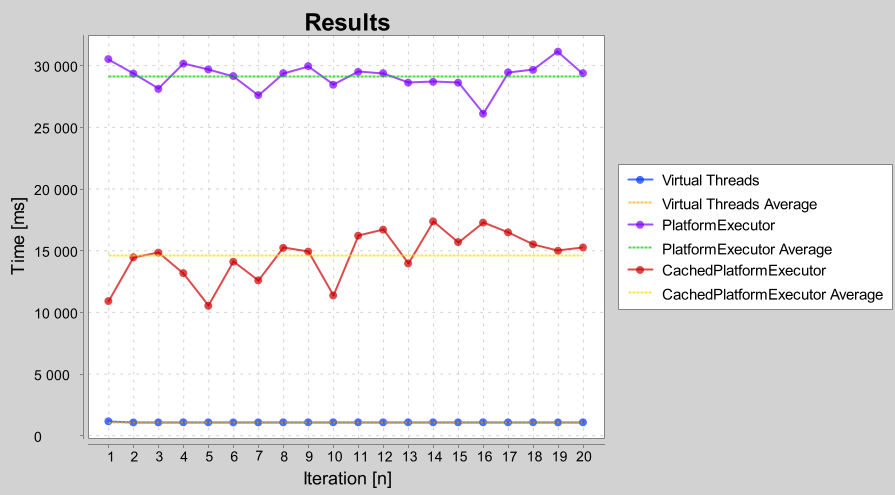
\includegraphics[width=1.0\textwidth]{sleep.png}
        \caption{Laufzeitmessungen bei wartenden Auslastung}
        \label{fig:sleep}
    \end{figure}
    Wie in der Abbildung \ref{fig:sleep} zu erkennen, fallen die Ergebnisse dieses Benchmarks sehr zugunsten der \Glspl{vt} aus. Sie benötigten im Durchschnitt  nur 1098.3845 ms. 
    Ein jeder Thread muss genau
    1000 ms warten. Daher wurden nur ca. 98 ms als Overhead benötigt um 100.000 \Glspl{vt} zu erstellen und zu verwalten. Daran, dass die Ausführungszeit einer jeden Iteration unter 2000 ms beträgt, ist
    erkennbar, dass alle Aufgaben parallel ausgeführt werden konnten.
    Der \texttt{CachedThreadPool} benötigte im Mittel 14588.2087 ms, also über das zehnfache länger als \Glspl{vt}.
    Sogar nochmal deutlich schlechter abgeschnitten hat der \texttt{ThreadPerTaskExecutor} mit einer mittleren Laufzeit von 29152.0905 ms. Somit war dieser nur etwa halb so schnell wie
    der \texttt{CachedThreadPool}. Aufgrund dieses hohen Unterschiedes ist anzunehmen, dass bei den beiden Benchmarks, die ausschließlich \Glspl{pt} nutzen, nicht alle Aufgaben parallel ausgeführt
    werden konnten. Der \texttt{CachedThreadPool} konnte die Laufzeit reduzieren, indem die Threads, die ihre Aufgaben abgeschlossen haben, wiederverwendet werden. Somit fällt in einigen Situationen 
    die ressourcenintensive Instanziierung weg. Sollten alle Threads gleichzeitig ausführbar sein, ginge dieser Vorteil verloren. Zusätzlich wurde auch ein \texttt{ForkJoinPool} getestet. 
    Im Punkt Laufzeit Schnitt dieser nur leicht besser als der \texttt{ThreadPerTaskExecutor} ab. Es ist auch anzumerken, dass 
    im Gegensatz zu allen anderen getesteten Thread-Pools beim \texttt{ForkJoinPool} nicht mehr mit dem Gerät interagiert werden konnte. Beim Versuch, im Hintergrund andere Prozesse auszuführen, kamen diese zum 
    Stillstand. 

\subsection{Laufzeitmessungen bei Abhängigkeiten zwischen Threads}
\label{subsec:LaufzeitmessungenbeiAbhängigkeitenzwischenThreads}

    Solch reine Anwendungsfälle, wie in den ersten beiden Benchmarks behandelt wurden, kommen in der Praxis natürlich nicht vor. Viel häufiger treten Mischfälle auf, in denen zwar teils rechenintensive Anweisungen
    ausgeführt werden,
    aber zusätzlich noch externe Abhängigkeiten eine Blockierung des Prozesses bewirken. Aus diesem Grund wird für einen weiteren Laufzeittest ein Produzenten-Konsumenten Modell herangezogen.
    Dabei platzieren eine Menge an Produzenten, die jeweils als ein eigener Thread implementiert sind, Objekte in eine \texttt{ArrayBlockingQueue} mit einer definierten maximalen Kapazität.
    Die Konsumenten entnehmen die Objekte wiederum aus der Warteschlange. Die \texttt{ArrayBlockingQueue} ist Thread-sicher implementiert und verhindert gleichzeitige Zugriffe. Außerdem werden 
    die Produzenten blockiert, sollte die maximale Kapazität erreicht werden. Dasselbe gilt für die Konsumenten sollte die Warteschlange leer sein. 
    Damit auch rechenintensive Operationen durchgeführt werden, rufen alle Konsumenten und Produzenten beim Ausführen ihrer Arbeitsschritte die Methode \texttt{executeNoneSense}, ersichtlich
    in Programm \ref{prog:ExecuteNoneSense} auf.

    \begin{figure}[H]
        \centering
        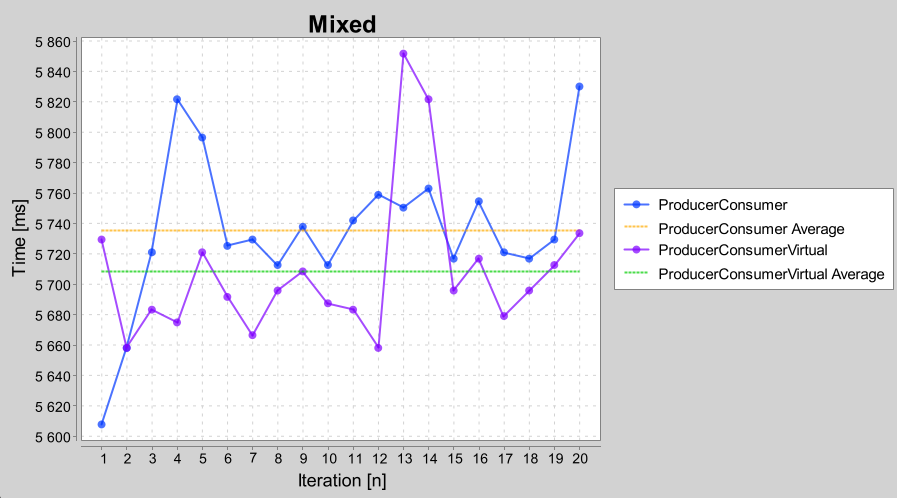
\includegraphics[width=1.0\textwidth]{mixed.png}
        \caption{Laufzeitmessungen bei Abhängigkeiten zwischen Threads}
        \label{fig:mixed}
    \end{figure}

    Die Abbildung \ref{fig:mixed} zeigt deutlich, dass der Unterschied zwischen den beiden Herangehensweisen eher gering ausfällt. Die Version mit den \Glspl{pt} benötigte im Durchschnitt 5735,2912 ms. 
    Die \Glspl{vt} waren in diesem Fall mit einer mittleren Ausführungsdauer von 5708,2711 ms um 1,5 \% schneller. Dies ist darauf zurückzuführen, dass die einzelnen Threads aufwändige Berechnungen 
    durchführen mussten bevor sie ein neues Element produzieren oder konsumieren konnten. Wären sehr viel mehr Threads dabei eingesetzt worden, die keine zusätzlichen Berechnungen durchführen müssten, wäre 
    dieser Benchmark mehr zugunsten der \Glspl{vt} ausgefallen.
    
\section{Messungen bei ScopedValues in verschiedenen Szenarien}
\label{sec:MessungenbeiScopedValuesinverschiedenenSzenarien}

    Da laut den Entwicklern und Entwicklerinnen von Projekt Loom die Klasse \texttt{ThreadLocal} in Kombination mit \Glspl{vt} zu Problemen beim Ressourcenbedarf führen kann, 
    wurden einige Messungen durchgeführt, die den Unterschied zwischen \texttt{ThreadLocal} und \texttt{Scoped\-Value} ermitteln sollen. Getestet wurden dabei verschiedene Szenarien
    unter der exklusiven Verwendung von \Glspl{vt}. 
    Als besonders schwierig stellte sich dabei die Ermittlung des Speicherverbrauchs dar, da die meisten Werkzeuge wie \texttt{MemoryMXBean} oder \texttt{org.github.jamm} die Neuerungen von 
    Projekt Loom noch nicht unterstützen.

\subsection{Laufzeit bei einzelnen Abfragen}
\label{sec:LaufzeitbeieinzelnenAbfragen}
    
    Ziel dieses Benchmarks ist es, die Klassen \texttt{ThreadLocal} und \texttt{ScopedValue} hinsichtlich Laufzeit bei einer Wertzuweisung und einer einzelnen Wertabfrage gegenüberzustellen.
    Dieses Szenario ist deswegen interessant, da bei der Verwendung von \texttt{ScopedValue} Caching erst bei wiederholten Abfragen zum Einsatz kommt. Bei der Nutzung von Thread-lokalen Variablen
    liegt der Wert immer direkt am Thread-Objekt selbst. 

    \begin{program} [H]
        \caption{Laufzeit bei einzelnen Abfragen}
        \label{prog:SingleQuery}
    \begin{JavaCode}[language=Java, numbers=left]
@BenchmarkMode(Mode.SampleTime)
@State(Scope.Thread)
@OutputTimeUnit(TimeUnit.SECONDS)
public class ScopedValueBenchmarkSingleQuery {
    private static final ScopedValue<String> sv = ScopedValue.newInstance();

    @Param({"100000"})
    private int numThreads;

    @Benchmark
    public void testScopedValue() throws Exception {
        try(var executor = Executors.newVirtualThreadPerTaskExecutor()) {
            for (int i = 0; i < numThreads; i++) {
                executor.execute(() -> ScopedValue.where(sv, "ScopedValue")
                .run(() -> { String value = sv.get(); }));
            }
        }
    }
}\end{JavaCode}
    \end{program}

    Wie in Programm \ref{prog:SingleQuery} zu sehen ist, wird in dem Beispiel eine einzelne Instanz der Klasse \texttt{ScopedValue} verwendet. Im Benchmark selbst wird ein Executor-Service benutzt, um eine
    in Zeile 7 definierte Anzahl an Threads zu starten, um den Einfluss externer Faktoren zu verringern. In jedem Thread geschieht eine Bereichs- und Wertzuweisung der Variable.
    Anschließend wird der Wert der Variable wieder abgefragt. Die Testklasse für \texttt{ThreadLocal} unterscheidet sich nur darin, dass ein \texttt{TreadLocal}-Objekt benutzt wird, um den Wert
    abzuspeichern.

    \begin{figure}[H]
        \centering
        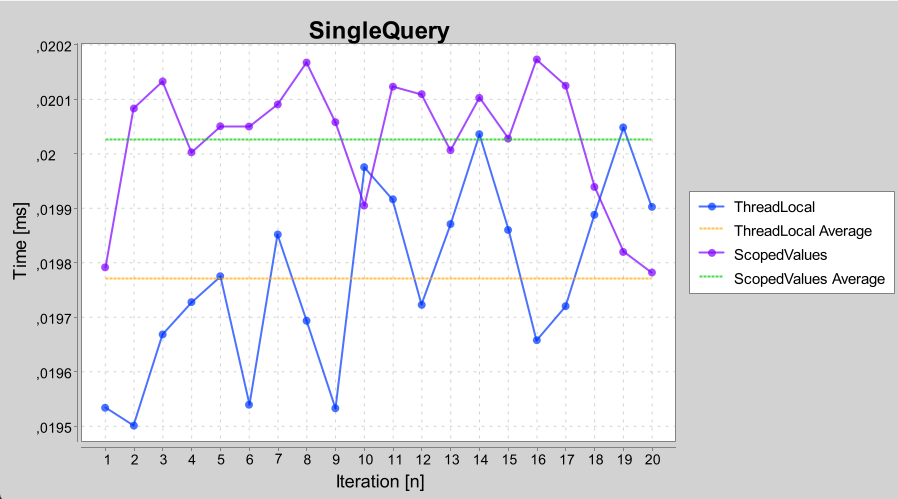
\includegraphics[width=1.0\textwidth]{SingleQuery.png}
        \caption{Laufzeitmessungen bei einzelnen Abfragen}
        \label{fig:SingleQuery}
    \end{figure}

    In \ref{fig:SingleQuery} ist zu erkennen dass der Unterschied zwischen den beiden Technologien in diesem Anwendungsfall gering ausfällt. Mit einer durchschnittlichen Ausführungsdauer von
    0,01977 ms war die Implementierung mit \texttt{ThreadLocal} um etwa 1,2 \% schneller als die Alternative. Die Implementierung mit \texttt{ScopedValue} benötigte im Mittel 0,02002 ms.
    Diese Messungen beinhalten auch die Zeit die benötigt wurde um die Objekte selbst zu erstellen und zu die Wertzuweisungen durchzuführen. Sollte dieser Vorgang bei einer der beiden Technologien 
    langsamer als bei der anderen erfolgen könnte dies dazu führen dass die Abfrage dafür um einiges schneller erfolgt als vermutet. Eine Berücksichtigung dieser Eigenschaft wäre für den praktischen
    Gebrauch wenig zielführend, da eine einzelne Wertabfrage ohne Wertzuweisung nicht durchführbar ist. 

\subsection{Laufzeit bei wiederholten Abfragen}
\label{sec:LaufzeitbeiwiederholtenAbfragen}

    Wie in Kapitel \ref{subsec:UnterschiedeScopedValuesundThreadLocal} bereits erwähnt, werden bereichsgebundene Variablen beim ersten Aufruf der Methode \texttt{get()} ebenfalls im Thread-Objekt 
    zwischengespeichert. Wenn dieser Zwischenspeicher nicht überfüllt wird, sollte dies zu einem Zuwachs der Zugriffsgeschwindigkeit führen. In diesem Testszenario wird dies überprüft.
    Die Testklasse selbst gleicht jener aus Programm \ref{prog:SingleQuery}. Der Unterschied liegt lediglich darin, dass in jedem Thread mehrere Zugriffe auf den Wert der Variable erfolgen. Eine 
    Wertzuweisung erfolgt hingegen ebenfalls wieder nur einmal zu Beginn.


    \begin{figure}[H]
        \centering
        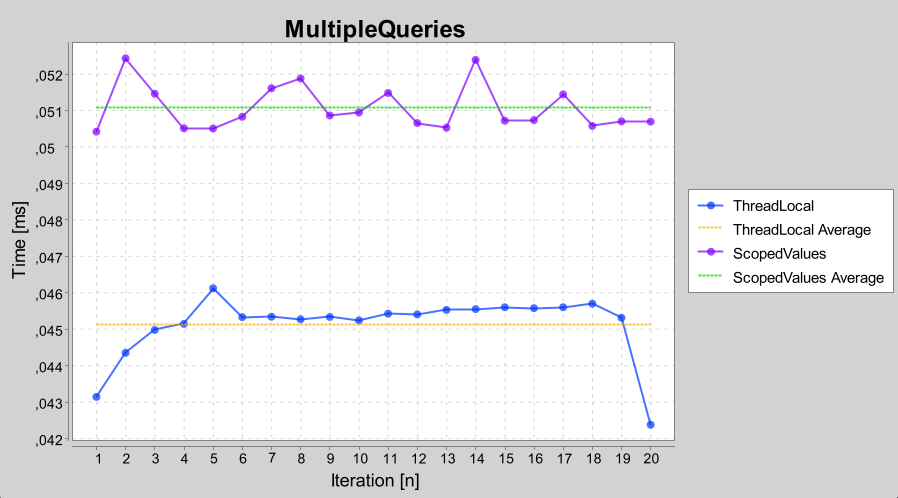
\includegraphics[width=1.0\textwidth]{MultQuery.png}
        \caption{Laufzeitmessungen bei wiederholten Abfragen}
        \label{fig:MultQuery}
    \end{figure}

    Der Fakt dass bei wiederholten Wertabfragen von bereichsgebundenen Variablen der Wert am Thread selbst zwischengespeichert werden sollte, lässt vermuten, dass der Unterschied zu Threadlokal 
    sehr gering ausfallen sollte. Dies ist in diesem Szenario, wie in Abbildung \ref{fig:MultQuery} zu sehen ist, nicht der Fall. Der Test für die Klasse \texttt{ThreadLocal} benötigte
    durchschnittlich 0,045122 ms. Der Test für \texttt{ScopedValue} benötigte mit 0,051074 ms etwa 13 \% mehr Zeit. Berücksichtigt man auch die Ergebnisse aus Kapitel \ref{sec:LaufzeitbeieinzelnenAbfragen}
    ist anzunehmen, dass bei der Klasse \texttt{ScopedValue} die Instanziierung und Wertbindung schneller erfolgt als bei \texttt{ThreadLocal}. Dafür benötigt die Wertabfrage mehr Zeit, auch bei einer 
    Zwischenspeicherung des Wertes direkt am Thread-Objekt.

\subsection{Laufzeit bei Thread-übergreifender Vererbung der Variablen}
\label{sec:LaufzeitbeiVererbung}
    Die Verhalten von \texttt{InheritableThreadLocal} wurde von den Entwicklern der \Glspl{vt} in Kombination mit einer hohen Anzahl an kurzlebigen Threads als potentiell problematisch 
    dargestellt. Diese Laufzeitmessung stellt daher den Vererbungsvorgang von \texttt{InheritableTreadLocal} und \texttt{ScopedValue} gegenüber.

    \begin{program} [H]
        \caption{Laufzeit bei Vererbung}
        \label{prog:Inheritance}
    \begin{JavaCode}[language=Java, numbers=left]
@BenchmarkMode(Mode.SampleTime)
@State(Scope.Thread)
@OutputTimeUnit(TimeUnit.SECONDS)
public class ScopedValuesInheritanceBenchmark {
    private static final ScopedValue<String> sv = ScopedValue.newInstance();

    @Param({"100000"})
    private int iterations;

    @Benchmark
    public void test(){
        ScopedValue.where(sv, "parent").run(() -> {
            try (var scope = new StructuredTaskScope<Void>()) {
                for (int i = 0; i < iterations; i++) 
                    scope.fork(() -> {int j = 0; return null; });
                scope.join();
            } catch (InterruptedException e) {
                throw new RuntimeException(e);
            }
        });
    }
}\end{JavaCode}
    \end{program}
    Da die threadübergreifende Vererbung eines bereichsgebundenen Wertes nur stattfindet, wenn der neue Thread durch die \texttt{fork}-Methode eines \gls{sts} erstellt wurde, wird eine Instanz 
    der Basisklasse \texttt{StructuredTaskScope} verwendet. Im neuen Thread selbst wird nicht mehr auf
    den Wert zugegriffen, da dieser Vorgang in den beiden Situationen unterschiedliche Performanz aufweisen können. Stattdessen wird eine einfache Instruktion mit einer konstanten Ausführungsdauer
    durchgeführt. Ein \gls{sts} erwartet bei jeder Teilaufgabe einen retournierten Wert, daher ist das zweite Statement in Zeile 15 nötig. Um eine \texttt{StructureViolationException} zu vermeiden,
    muss sich der gesamte \gls{sts} im Gültigkeitsbereich einer Wertbindung des \texttt{ScopedValue} befinden, auch die Instanziierung und der \texttt{join()}-Aufruf. Die Vergleichsmessung
    nutzt eine Instanz der Klasse \texttt{InheritableTreadLocal}. In Zeile 12 wird der Wert mittels der \texttt{set()}-Methode festgelegt.

    \begin{figure}[H]
        \centering
        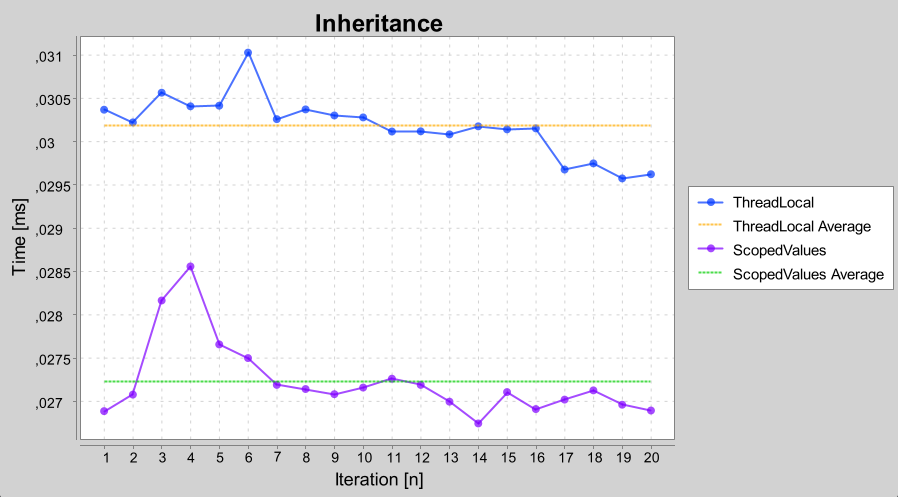
\includegraphics[width=1.0\textwidth]{Inheritance.png}
        \caption{Laufzeitmessungen bei Vererbung}
        \label{fig:inheritance}
    \end{figure}

    Der Test für bereichsgebundenen Werte benötigte in diesem Szenario im Durchschnitt 0.02723 ms. Die Ausführung der Version mit \texttt{ThreadLocal} war mit 0.03018 ms um etwa 10 \% langsamer. 
    Bei Threads mit einer sehr kurzen Lebensdauer könnte dieser Geschwindigkeitsunterschied bedenklich sein, wobei vorher abgewogen werden sollte, ob eine Vererbung der Werte überhaupt 
    benötigt wird. Bereichsgebundene Variablen können zwar beschleunigen, doch die Auswahl sollte anhand der benötigten Eigenschaften erfolgen, wie beispielsweise der Veränderbarkeit.

\subsection{Speicherbedarf bei einer hohen Anzahl an Threads}
\label{sec:Speicherbedarf}

    Interessant ist ebenfalls die Gegenüberstellung der beiden Technologien bei ihrem Speicherbedarf. Dazu wird ein \texttt{byte}-Feld mit 1.048.576 Einträgen erstellt und als Wert für einen
    \texttt{ScopedValue} benutzt. Dieser Wert wird dann auf 1000 neue \Glspl{vt} vererbt. Dazu kommt ein \gls{sts} zum Einsatz. Direkt vor und nach dem \gls{sts} wird mittels 
    \texttt{MemoryMXBean} der von der \gls{jvm} verwendete Speicher ermittelt. Nach kurzem Warten und einem Aufruf von \texttt{System.gc()}, um den Garbage-Collector zu aktivieren, wird 
    dieser Vorgang für \texttt{InheritableThreadLocal} wiederholt. Nach 5 Messiterationen konnte festgestellt werden, dass \texttt{InheritableThreadLocal} einen 137-fachen Speicherbedarf 
    vorweist, obwohl in jedem Thread ein Zugriff auf den Wert durchgeführt wurde, damit das Caching bei \texttt{ScopedValue} durchgeführt werden kann. Dieses Verhalten weist darauf hin, dass
    das Zwischenspeichern des Wertes am Thread-Objekt bei \texttt{ScopedValue} in diesem Fall nur begrenzt oder gar nicht durchgeführt wurde. Auch wenn die Methode zur Ermittlung des Speicherbedarfs 
    nicht unbedingt präzise ist, stellt sich das Ergebnis als so aussagekräftig heraus um einen Schluss ziehen zu können. Sollten viele Thread benötigt werden und der bereitgestellte Wert 
    nicht in jedem Thread benötigt werden stellt sich \texttt{ScopedValue} als wesentlich speichersparender heraus. Der Quelltext ist im Anhang in Programm \ref{prog:Speicherverbrauch} zu finden.

\chapter{Zusammenfassung und Fazit}
\label{cha:fazit}
    Projekt Loom stellt einige Neuerungen für die Sprache Java vor. Vor allem im Bereich der Nebenläufigkeit wird die Sprache erweitert. Das Herzstück dabei stellen die Virtual-Threads (VT) dar.
    Dabei handelt es sich um flexible, leichtgewichtige Threads, die geringere Laufzeitkosten bei der Instanziierung vorweisen. Dadurch können sie schneller und in größeren Mengen erstellt werden.
    Sie führen ihre Aufgaben auf einem Plattform-Thread (PT) aus, von dem sie bei Bedarf wieder gelöst werden können. Somit werden sie im Gegensatz zu \Glspl{pt} von der \gls{jvm} verwaltet.
    Im Vergleich zu \Glspl{pt} weisen \Glspl{vt} wenig Nachteile auf. Lediglich bei wenigen, stark rechenintensiven Aufgaben ganz ohne blockierende Aufrufe sollten \Glspl{pt} bevorzugt werden, da \Glspl{vt}
    in diesem Fall einen kleinen Overhead verursachen. In den meisten Fällen ist dieser aber vernachlässigbar. Sollten Threads kurzlebig sein oder in großen Mengen benötigt werden, sind \Glspl{vt}
    wegen ihrer Leichtgewichtigkeit und der hohen Verfügbarkeit definitiv
    zu bevorzugen. Auch bei Aufgaben, die oft blockiert werden, sollten sie eingesetzt werden. In der Verwendung unterscheiden sie sich von \Glspl{pt} 
    meist nur bei der verwendeten Factory-Methode zum Erzeugen eines Thread-Objektes und können wie gewohnt benutzt werden.
    Somit können sie in fast allen Fällen getrost anstatt \Glspl{pt} eingesetzt werden. Andere Probleme der nebenläufigen Programmierung wie "Deadlocks" oder "Race-conditions" werden durch \Glspl{vt} nicht gelöst.
    Mit diesen Schwierigkeiten muss sich weiterhin der Anwender plagen.

    StructuredTaskScopes (STS) sollen die Handhabung von nebenläufigen Aufgaben vereinfachen und strukturieren. Dabei geht es darum, eine Menge an ähnlichen Teilaufgaben als eine Einheit zu koordinieren. Dabei können allgemeine
    Ausführungslogik und Fehlerbehandlung festgelegt und wiederverwendet werden, indem man von der Basisklasse \texttt{StructuredTaskScope} ableitet und meist einfache Anpassungen vornimmt. Ein einziger Methodenaufruf wartet auf
    die Beendung aller Teilaufgaben.
    Diese Eigenschaften können mit Thread-Pools nur
    schwer erreicht werden.Da im Hintergrund \Glspl{vt} benutzt werden,
    ist eine gute Skalierbarkeit gegeben. Außerdem stellen sie derzeit die einzige Möglichkeit dar, threadübergreifende Vererbung bei \texttt{ScopedValue}s zu erreichen.

    \texttt{ScopedValue}s ermöglichen die Bindung von Werten an einen Wertebereich, auch über Methodengrenzen hinweg. Im Gegensatz zu \texttt{ThreadLocal} sind diese Werte nicht veränderbar, was zu einer 
    besseren Struktur und leichter lesbarem Code führen kann. Alternativ kann der Wert in einem neuen Bereich überschrieben werden. Der Wert wird nach Verlassen des Bereichs auch wieder freigegeben und
    benötigt keine weitere Aufmerksamkeit. Im direkten Vergleich zu \texttt{ThreadLocal} sind sie bei der Wertabfrage zwar langsamer, stellen sich aber bei einer threadübergreifenden Vererbung als schneller heraus.
    Zusätzlich benötigen sie bei großen Mengen an Threads wesentlich weniger Speicher und sind daher für die Verwendung in Kombination mit \Glspl{vt} sehr zu empfehlen. 
% \chapter{Die Abschlussarbeit}
\label{cha:Abschlussarbeit}


% \chapter{Zum Arbeiten mit \latex}
\label{cha:ArbeitenMitLatex}


% \chapter{Abbildungen, Tabellen, Quellcode}
\label{cha:Abbildungen}



% \chapter[Mathem.\ Formeln etc.]{Mathematische Formeln, Gleichungen und Algorithmen}
\label{cha:Mathematik}


% \chapter[Umgang mit Literatur]{Umgang mit Literatur und anderen Quellen}
\label{cha:Literatur}


\cite{Drake1948}	% eine Quelle als Test



% \chapter{Drucken der Abschlussarbeit}
\label{cha:Drucken}


% \chapter{Schlussbemerkungen}
\label{cha:Schluss}



%%%-----------------------------------------------------------------------------
\appendix                                                               % Anhang 
%%%-----------------------------------------------------------------------------

\chapter{Technische Informationen}
\label{app:TechnischeInfos}


% \chapter{Ergänzende Inhalte} % \chapter{Inhalt der CD-ROM/DVD}
\label{app:materials}


Auflistung der ergänzenden Materialien zu dieser Arbeit, die zur digitalen Archivierung an der 
Hochschule eingereicht wurden (als ZIP-Datei).

% Nur als Beispiel, die Struktur sollte man an die eigenen Bedürfnisse anpassen!

\section{PDF-Dateien}
\begin{FileList}{/}
\fitem{thesis.pdf} Finale Master-/Bachelorarbeit (Gesamtdokument)
\end{FileList}

\section{Mediendaten}
\begin{FileList}{/media}
\fitem{*.ai, *.pdf} Adobe Illustrator-Dateien
\fitem{*.jpg, *.png} Rasterbilder
\fitem{*.mp3} Audio-Dateien
\fitem{*.mp4} Video-Dateien
\end{FileList}


\section{Online-Quellen (PDF-Kopien)}
\begin{FileList}{/online-sources}
\fitem{Reliquienschrein-Wikipedia.pdf} {\backtrackerfalse\parencite{WikiReliquienschrein2023}}
\end{FileList}
 % Inhalt der CD-ROM/DVD
% \chapter{Fragebogen}
\label{app:Fragebogen}

 % Chronologische Liste der Änderungen
% \chapter{\latex-Quellcode}
\label{app:Quellcode}

 % Quelltext dieses Dokuments

%%%-----------------------------------------------------------------------------
\backmatter                          % Schlussteil (Quellenverzeichnis und dgl.)
%%%-----------------------------------------------------------------------------

\MakeBibliography % Quellenverzeichnis

%%%-----------------------------------------------------------------------------
% Messbox zur Druckkontrolle
%%%-----------------------------------------------------------------------------

% \chapter*{Messbox zur Druckkontrolle}



\begin{center}
{\Large --- Druckgröße kontrollieren! ---}

\bigskip

\calibrationbox{100}{50} % Angabe der Breite/Hoehe in mm

\bigskip

{\Large --- Diese Seite nach dem Druck entfernen! ---}

\end{center}



%%%-----------------------------------------------------------------------------
\end{document}
%%%-----------------------------------------------------------------------------
